%{{{ preamble
% Note: The order of some of these packages are important.
% fleqn left alligns all equations. Using settings from uiophd.cls.
\documentclass[altfont, fleqn]{uiophd}
\usepackage[T1]{fontenc}
\usepackage[utf8]{inputenc}
\usepackage[usenames,dvipsnames,svgnames]{xcolor}			
% Rebinds commands safer than using \let\mycref\cref.
\usepackage{letltxmacro}
% Can change properties of sections, such as color. 
\usepackage{titlesec}		
% Adds customizable headers and footers. 
\usepackage{fancyhdr}		
% Adds small toc lists. 
\usepackage{titletoc}		
\usepackage{hyperref}
\usepackage{graphicx}
% Essential math package.
\usepackage{amsmath}		
% \abs and \norm.
\usepackage{commath}		
% Do not know.
\usepackage{textcomp}
% SI units package.
\usepackage[redefsymbols=false]{siunitx}		
% Some extra signs and other fonts.
\usepackage{bm,upgreek} 
\usepackage{appendix}
\usepackage[
	backend=biber,
    style=authoryear,
    citestyle=authoryear,
	doi=false,
	maxcitenames=2,
]{biblatex}
% Place figures inline with text.
\usepackage{wrapfig}
% Have to import this at the end for this to work somehow.
\usepackage{cleveref}		
\usepackage{multicol}
% Caption options. Used to change label color.
\usepackage{caption}
% Commands that help placing figures side by side.
\usepackage{subcaption}
% Used with minted to get caption on top.
\usepackage{floatrow}
% Highlighting of source code.
\usepackage{mdframed}
\usepackage{minted}
\usemintedstyle{manni}
\floatsetup[listing]{style=Plaintop}
% \surroundwithmdframed{minted}
% \BeforeBeginEnvironment{minted}{\begin{mdframed}}
% \AfterEndEnvironment{minted}{\end{mdframed}}
    
%%%% BUGFIX in titlesec%%%%
\usepackage{etoolbox}
\makeatletter
\patchcmd{\ttlh@hang}{\parindent\z@}{\parindent\z@\leavevmode}{}{}
\patchcmd{\ttlh@hang}{\noindent}{}{}{}
\makeatother
%%%% END BUGFIX %%%%

\addbibresource{master.bib}

% Remove certain fields from appearing in the bibliography.
\AtEveryBibitem{\clearfield{month}}
\AtEveryBibitem{\clearfield{day}}
\AtEveryBibitem{\clearfield{note}}
\AtEveryCitekey{\clearfield{month}}
\AtEveryBibitem{%
    \ifentrytype{misc}
    {%
    }%
    {%
        \clearfield{url}
        \clearfield{urldate}
    }%
}

% Use ampersand "&" instead of "and". 
\renewcommand*{\finalnamedelim}{%
    \ifnumgreater{\value{liststop}}{2}{\finalandcomma}{}%
    \addspace\&\space%
}
% Paper properties. 
\pagestyle{fancy}
% Removes the header bar and text.
\renewcommand{\headrulewidth}{0pt}
\fancyhead{}
% Custom colors.
\definecolor{viridis_01}{rgb}{0.267004, 0.048740, 0.329415}
\definecolor{viridis_02}{rgb}{0.190631, 0.407061, 0.556089}
\definecolor{viridis_03}{rgb}{0.208030, 0.718701, 0.472873}
\definecolor{viridis_04}{rgb}{0.993248, 0.906157, 0.143936}
% Change section formatting.
\titleformat{\section}
    {\color{viridis_02}\Large\bfseries}
    {\color{viridis_02}\thesection}{1em}{} 		
% Change section formatting.
\titleformat{\subsection}
    {\color{viridis_02}\large\bfseries}	
    {\color{viridis_02}\thesubsection}{1em}{}

% Change chapter formatting.
\titleformat{\chapter}[hang] 				
    {\bfseries\Huge} 	
    {\color{viridis_01}\thechapter\hspace{20pt}\rule[-3pt]{2pt}{23pt}\hspace{10pt}}
    {0.5ex} 			
    {\color{viridis_01}} 	
    [
    ]		
% Change the color of every citation.
\AtEveryCite{\color{viridis_03}}
% Hyperlink colors. 
% Empty color disables coloring.
\hypersetup{
	colorlinks=true,
	citecolor=viridis_03,
	filecolor=black,
	linkcolor={},
	urlcolor=black,
}

% Change the color of caption labels.
\captionsetup{labelfont={color=viridis_03}}

% Change color of clever ref.
\AtBeginDocument{
    \LetLtxMacro{\mycref}{\cref}
	\renewcommand{\cref}[1]{{\color{viridis_03}\mycref{#1}}}
    \LetLtxMacro{\myCref}{\Cref}
	\renewcommand{\Cref}[1]{{\color{viridis_03}\myCref{#1}}}
    \LetLtxMacro{\mynameref}{\nameref}
	\renewcommand{\nameref}[1]{{\color{viridis_03}\mynameref{#1}}}
    % \LetLtxMacro{\myfullref}{\fullref}
	% \renewcommand{\fullref}[1]{{\color{viridis_03}\myfullref{#1}}}
}
% % Change the spacing of some math symbols in math mode.
% \setlength{\thickmuskip}{6pt}
%}}} end of preamble
\begin{document}
%{{{ Abstract
\chapter*{Abstract}
\noindent
% The physical processes that creates electrical signals in neurons are well understood, 
% but how the signals are processed into actions and thoughts has yet to 
% receive a robust answer
% Cell type classification is of high importance because the function of different 
% neurons is still largely a mystery. 

% Optimal Spike widht
% Optimal spike amplitude
% Amplitude gives better seperation between classes. 
% It works under filter. 
Duration of intracellular spikes has long been an indicator 
of pyramidal neurons versus interneurons. 
Using NEURON and LFPy spike width and amplitude measurements from
\Textcite{pettersen_amplitude_2008}
using the Hay model
were replicated.
To investigate how spike amplitude
and width can classify pyramidal neurons and interneurons,
measurements were done 
in 260 biophysical models
from the Blue Brain Project. 
1000 electrodes were positioned randomly around each soma to mimic
experemental procedures.
Probability distributions of the measured widths and amplitudes
were compared using AOC curves and a overlap measure. 
The spike width definitions were found to considerably effect
how well classification can be done with 
the peak-to-peak spike width definition providing the best results. 
When the spike width combined with spike amplitude 
significantly increased 
the seperation between
interneuron and pyramidal neurons.
This suggests that areas in the spike amplitude width space 
can be attributed to certain kinds of cell types. 
When a butterworth filter were applied to the spike shapes
the seperation between interneuron and pyramidal neurons remained
showing that classification can still be done using the filtered 
signals. 

%}}} end of Abstract
%{{{ Table of Contents
\setcounter{tocdepth}{1}
\startcontents
\tableofcontents
%}}} end of Table of Contents
%{{{ Introduction
\chapter{Introduction}

% Since 
% the conception of neuroscience the neurons function have been studied on many levels
% from the properties of the cell membrane to clustered networks of neurons.

Early research showed that interneurons that high firing rates
showed "thin" action potentials with short durations. 
These action potentials could be distinguised from pyramidal 
cells with longer action potentials and showed a 
more regular spiking pattern
(\textcite{mountcastle_cortical_1969}).
Pyramidal cells excibiting long and regular spike patterns
has since been refered to as regular spiking. 
These difference between these spike shapes were 
thouroughly examined in brain slices from rodents. 



% TODO: COPY Vigneswaran.
% Early investigators first suggested that
% interneurons, with high spontaneous firing rates, had “thin” ac-
% tion potentials of short duration and could be distinguished from
% pyramidal cells with longer action potentials and lower, regular
% spiking pattern of discharge (Mountcastle et al., 1969). These
% differences were subsequently confirmed by detailed intracellular
% studies in brain slices from rodents (Connors et al., 1982; McCor-
% mick et al., 1985; Contreras, 2004).

% There are several types of neurons 
% and it was early noticed that the discharge waveform
% had different shapes
% for different types on neurons.
%TODO: Source

% The behaviour of neuronal circuits is heavily effected by the kinds of neurons
% it has. 
% Investigating the different kinds of is therefor of major importance. 
% The majority of studies that use  extracellular recordings ignore 
% neuronal types, while some studies have attempted to classify
% neurons based on signal waveforms and spike patterns. 
% TODO: SOURCE

% TODO: COPY katai
% Intracellular recordings in slice
% preparations have demonstrated that c-aminobutyric acid (GABA)-
% containing, inhibitory interneurons produce action potentials of a
% much shorter duration than excitatory, pyramidal neurons (McCormick
% et al., 1985).

% TODO: COPY katai
% Based on this finding, some extracellular recording
% studies distinguished neuronal types based mainly on the differences
% in spike width (Wilson et al., 1994; Constantinidis \& Goldman-Rakic,
% 2002; Mitchell et al., 2007; Cohen et al., 2009).
% However, the identification of neuronal types by their spike width
% alone has several problems. First, in extracellular recording conditions,
% the measurement of spike width is often disturbed by background
% noise near the baseline and the filtering parameters used in the
% experiment. Second, it has become clear that not all short-duration
% action potentials are generated by fast spiking (FS) interneurons.
% Intracellular studies have documented short-duration action potentials
% in a number of neurons that were subsequently labeled and shown to
% have a pyramidal morphology (Nowak et al., 2003).

% In addition measurements from some pyramidal axons has been shown
% to give shorter duration action potentials (Robbins 2013).
%(Vigneswaran 2011).

% TODO: COPY Bartho 2004
% In the hippocampus, the combination of several extracellular
% features, such as spike duration, firing rate, and pattern and
% spike waveform, reliably separates pyramidal cells from inter-
% neurons (Csicsvari et al. 1999). The validity of neuron classi-
% fication on the basis of extracellular features has been sup-
% ported by in vivo intra- and juxtacellular labeling as well as
% simultaneous extra- and intracellular recordings from the same
% neurons (Henze et al. 2000; Klausberger et al. 2003; Sik et al.
% 1995). Similar classification criteria are not available in the
% neocortex. Mountcastle et al. (1969) have noted that the occa-
% sionally recorded “thin spikes” in the somatosensory cortex
% had different response properties than the majority of units and
% suspected that they were interneurons. Other observations in-
% dicated that fast-spiking neurons have receptive and evoked
% response properties different from the majority of slower, more
% regular firing cells (Constantinidis and Goldman-Rakic 2002;
% Simons 1978; Swadlow 2003; Swadlow and Gusev 2002;
% Swadlow and Lukatela 1996; Swadlow et al. 1998). Intracel-
% lular recordings and labeling in cortical slices showed numer-
% ous classes of interneurons on the basis of the firing rates, spike
% morphology, and spike dynamics (Connors et al. 1982; Gupta
% et al. 2000; Kawaguchi and Kubota 1993; Somogyi et al.
% 1998). However, the information gathered in intracellular ex-
% periments in vitro cannot be directly applied to extracellularly
% recorded spikes in the intact brain. Furthermore, intra- and
% juxtacellular studies carried out in vivo do not directly support
% the suggestion that fast firing neurons unequivocally identify
% interneurons (Azouz et al. 1997; Degenetais et al. 2002; Doug-
% las et al. 1995; Gray and McCormick 1996; Steriade et al.
% 1998).

% Another popular approach is classifying based on discharge patterns, 
% such as bursting behaviour and inter spike interval (ISI).
% Classification based on inter spike bursting behavior and ISI has
% gained more traction than soley using spike waveform. 
% % Though classification based on discharge pattern has been accepted
% % as a better method than using the waveform, 

% These classifications are often based
% on the response of a current pulse which makes them difficult
% to apply on recordings from
% in vivo measurements. 
% % Taking another approach, recent intracellular recording studies have
% % revealed that cortical neurons can be classified into four types by their
% % discharge patterns in response to current pulses 
% (Kang \& Kayano,
% 1994; Gray \& McCormick, 1996; Nowak et al., 2003; González-
% Burgos et al., 2004, 2005a,b).

% % The problem
% % While doing single cell recordings the only information
% % about the neuron that is avaiable is the electric signal from the neuron.
% Modern types of 
% classification uses genotype?, the structure of the neuron and the 
% electric signal.

% While doing single cell recordings on alive subjects the researchers are
% recording in the dark. 

% In this article we show that interneurons can be seperated from pyramidal
% neurons based on data and models from the Blue Brain project. 
% The program makes an easy way to do the same analysis
% on future models as long as the models can be loaded with LFPy.


%}}} end of Introduction
%{{{ Theory
\chapter{Theory}
% NOTE: 
% The physical processes in and around neurons are well understood in comparison
% to the function they serve. 
% The basic function of a neuron is to receive and send 
% action potentials, 
% but what exact information is being transmitted or how 
% it is processed into thoughts does still not have a conclusive answer.

\vspace{1em} 
\startcontents
\printcontents{}{1}{\setcounter{tocdepth}{2}}
  
%{{{ The Neuron
\section{The Neuron}
\begin{figure}[h]
    \centering
    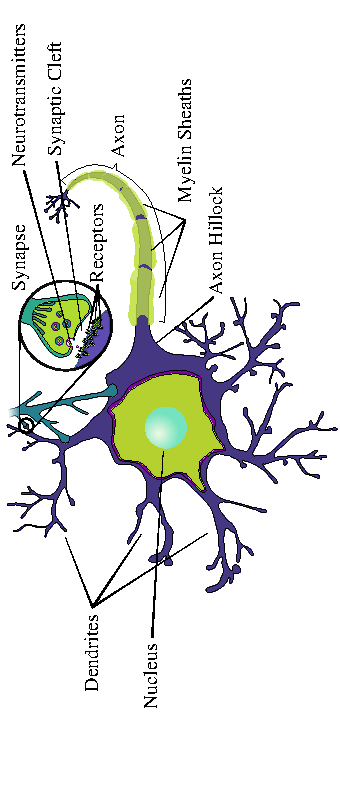
\includegraphics[angle=-90,width=1.0\textwidth]{images/2_1/neuron_structure.pdf}
    \caption{}
    \label{fig:2_1_neuron}
\end{figure}
\noindent
Neurons 
are electrically excitiable cells
that are a fundamental part of all brain functions.
Other names include {nerve cells}, {neurone} or more 
colloquially {brain cells}.
Neurons form in big networks 
which process information,
and in the human brain there is an estimated $10^{11}$ neurons.

Special proteins in the cell membrane enables the neuron to
fire action potentials when it is electrically excited. 
These action potentials are sharp voltage changes that propagates through
the full structure of the neuron.
The same properties that makes the neuron able to fire makes 
the action potential {regenerative}, meaning it will propagate
without decay.

The body of the neuron, the {soma}, has {dendrites} and 
the axon attached to it. 
The dendrites and the axon are very thin branching structures 
with a width usually in the order of \SI{1}{\micro\metre}. 
While neurons often have many dendrites directly attached to the soma
there is only one axon attached to the soma at the axon hillock.
The axon can branch several times before it ends and 
usually connects to the dendrites of other neurons via synapes.

The synapes are electrically sensitive which allows information
to pass between neurons. 
Though the majority of all synapes are axo-dendritic 
(axon to dendrite),
other junctions are also possible.
Other junctions include but are not limited to,
dendrite to dendrite, 
axon to axon and 
axon to blood vessel. 
When an action potential reaches a synapse it will activate
the synapse and pass information to the connect neuron. 
The information that is passed along depends on the type of synapse,
and if it is of a chemical or electrical type.

% TODO: Copy
The neocortex represents the great majority of the cerebral cortex. 
It has six layers and contains between 10 and 14 billion neurons. 
The six layers of this part of the cortex are numbered with Roman numerals 
from superficial to deep. Layer I is the molecular layer, which contains 
very few neurons; layer II the external granular layer; 
layer III the external pyramidal layer; layer IV the internal 
granular layer; layer V the internal pyramidal layer; and layer VI the 
multiform, or fusiform layer. Each cortical layer contains different neuronal 
shapes, sizes and density as well as different organizations of nerve fibers.

% NOTE: Topic to mention:
% Neuron cell types, pyramidal neurons, basket neurons interneurons, what 
% are they. The term "morphology". Intracellular also referred to as membrane potential.
% Subcortical. Se hemalainen p.421. for a good summary. What is transmembrane current. 
% Impulse. Apical dendrites. Grey matter. Spines. Synapses. Quiescent neuron.

%}}} end of The Neuron
%{{{ Electrical Activity
\section{The Cell Membrane}
\begin{figure}[h]
    \centering
    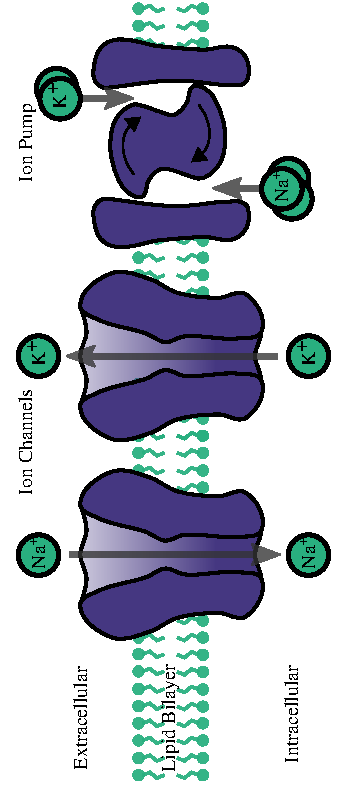
\includegraphics[angle=-90,width=1.0\textwidth]{images/2_1/ion_pumps_0.pdf}
    \caption{
        Common portrayal of ion channels and pumps in the neuron cell membrane. 
        They are responsible for
        creating a potential gradient across the membrane. 
        Ion channels have
        selective permeability of ions. Ion pumps activly transport ions
        through the membrane, often against the potential gradient. 
        Image modified from 
        \textcites{sterratt_principles_2011}.
    }
    \label{fig:2_ion_channels}
\end{figure}
The potential difference between the inside and outside the neurons 
are caused by different concentrations of 
ions
in the extracellular and intracellular medium. 
The ions cannot pass through 
the cell membrane as it
consists of a \SI{5}{\nano\metre} lipid bilayer which is mostly impenetrable 
to ions. 

In the membrane sits ion channels and 
ion pumps which can have selective permeability to ions. 
Collectivly they are refered to as ion transporters. 
These are created by proteins in complicated shapes. 
There and there are over 200 
kinds of electrically sensitive ion channels.
Together they create a 
potential gradient across the membrane. 
The most significant ions in this process are Sodium (Na$^+$), Potassium (K$^+$), 
Calcium (Ca$^{2+}$), Magnecium (Mg$^{2+}$) and Chloride (Cl$^{-}$). 
Ion channels are divided between passive channels and 
active channels where the active channels can change 
permeability under certain conditions while passive channels have a constant
permeability. 
\Cref{fig:2_ion_channels} shows a common portrayal of ion channels and pumps. 

The ion pumps differ from the channels by activly transporting certain
ions through the membrane. 
For instance, the Sodium-Pottasium exchanger pushes two K$^+$ ions out of the cell
for every three Na$^+$ it pushes into the cell. Doing this creates a net 
loss of charge inside the cell and the pump is therefore electrogenic. 
Not all pumps are electrogenic, the Sodium-Hydrogen exchanger transports
H$^+$ and Na$^+$ without effecting the net charge.
For each H$^+$ ion out of the cell the pump pushes one Na$^+$
into the cell. 

To further understand the electrical activity of neurons it is useful
to view the neuron as an electronic circuit where the ion channels, ion pumps
and the membrane serve as different electronic components.
\Cref{fig:2_hud_hux} shows the electronic circuit used by hudgkin
and huxley in their original description of a neuron membrane. 
\textcites{hodgkin_quantitative_1952, sterratt_principles_2011}

\begin{figure}[h]
    \centering
    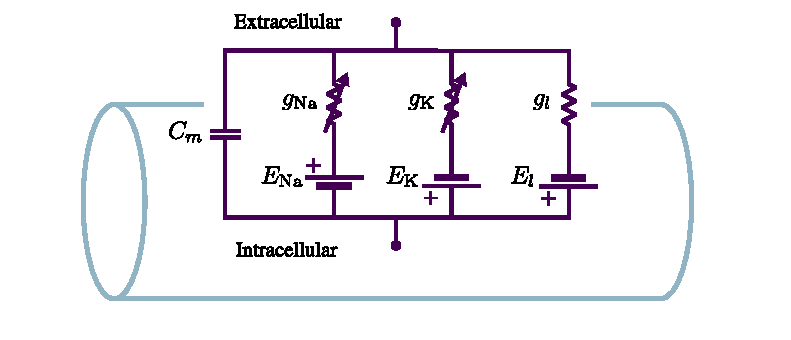
\includegraphics[width=1.0\textwidth]{images/2_1/compartment.pdf}
    \caption{Hodgkin and Huxley electrical circuit. 
    Circuit model of a neuron membrane. 
    Each ion channel sets up a potantial like a battery with the 
    selective permiability of ions represented by a variable resistor. 
    }
    \label{fig:2_hud_hux}
\end{figure}

% The temperature is important.
%}}} end of Neuronal Models
%{{{ Ciruit Model 
\section{Circuit Model}
Hudgking and Huxley originally tried to understand the
electrical properties of neuron by studing squid axons. 
Given spesific functions for the active conductances $g_\text{Na}$
and $g_\text{K}$, this circuit is enough to describe an important feature
of neurons, called action potentials.
Alan Hodgkin and Andrew Huxley got the nobel price for their
research on the biophysics of action potentials. 

The current equation of this neuronal equivalent circuit is
$$I = C_m \frac{dV}{dt} + I_\text{Na} + I_\text{K} + I_\text{l}.$$




% The model was developed by recording the activity of each
% type channel in the membrane. 
% The model of each channel was then constructed by fitting 
% the data to functions. 
% The final model of the cell membane was then constructed 
% by incorperating each channel model. 

%}}} 
%{{{ Action Potential
\section{Action Potential}
Action potentials are sharp increases in the membrane potential
followed by a less sharp decrease towards the resting potential. 
They are generally accepted as the information carriers between neurons
and as such has been a big focus of neuroscience since its discovery.

The shape of the action potentials are directly 
related to the types and densities
of the ion channels present in the membrane. 
This makes the action potential from neurons to look slightly differnt, 
though they all have common features. 
\Cref{fig:2_action_potential_anatomy} shows the anatomy of an action potential and some common definitions. 
\begin{figure}[h]
    \centering
    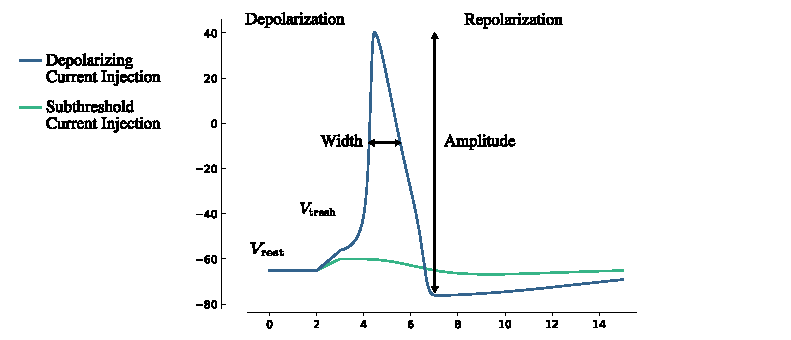
\includegraphics[width=\textwidth]{images/sec_2/action_potential.pdf}
    \caption{
    }
    \label{fig:2_action_potential_anatomy}
\end{figure}

In the the depolarization phase the potential rises towards the peak magnitude, 
while in the repolarization phase the potential decreases towards
the cells resting potential.
When the potental is below the resting potential 
it reaches the afterhyperpolarization phase before
it returns to its resting potential.

%}}} end of Action Potential
% Neuron Models {{{ %
\section{Multi Compartmental Models}
The circuit model represents a patch of a neuronal membrane
where the potential across the membrane is the same. 
If we want to study the voltage change across a longer piece of 
membrane we want to divide the membrane into parts and have a model for
each of them. 
This is the basis for creating bigger models, where multiple pices
of membrane equivalent circuits are combined into a multi-compartmental
model. 
The size of the compartments are small enough that the membrane potential is
considered the same at all places. 

\begin{figure}[h]
    \centering
    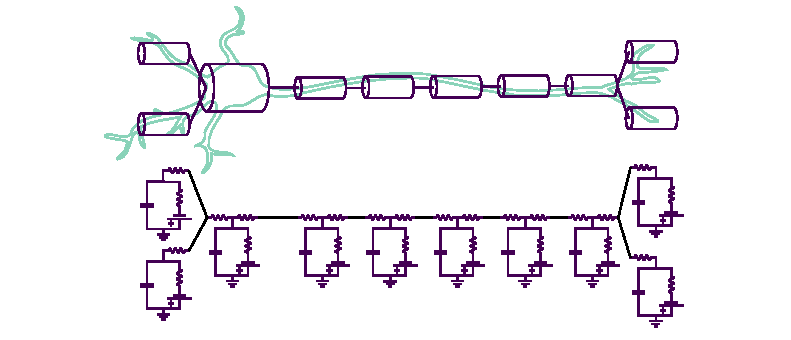
\includegraphics[width=1.0\textwidth]{images/2_1/compartments.pdf}
    \caption{Compartmental model.}
    \label{fig:2_comp_mod}
\end{figure}
% }}} 
%{{{ Electrodes
\section{Electrodes}
In most cases the membrane potential is wanted when measuring neurons. 
Though recording the membrane potental is not always feasable, 
especially in living subjects. 
Most knowledge about the physiological function of the brain is 
based on the recordings from single point electrodes. 

There are several types of electrodes and are always improving
in quality. 
Earlier studies were often limited by the precision of the instruments. 
The type of electrodes used depends on several factors. 
An often used type of electrode are tetrodes consisting of 
four very small electrodes bundled together. 
The size of each electrode is generally around
\SI{30}{\micro\metre} in diameter. 

Raw data from electrodes are usually band pass
filtered to remove unwanted noise from the signal. 
A big source of noise come at low frequencies below about 
\SI{300}{\hertz}
comes from populations of neurons firing. 
This band of frequencies are sometimes refered to as the local field
potential. 

% % TODO: Copy
% A tetrode is a type of electrode used in neuroscience for electrophysiological 
% recordings. 
% Tetrodes are constructed by bundling together four very small electrodes; 
% each wire is generally less than 30 μm in diameter. 
% Tetrodes are used to classify extra-cellular action potentials into sets generated 
% by the individual neurons, as each channel of the tetrode is usually close enough 
% to a cell such that action potentials emitted by that cell are detected on each of 
% the four channels, but because of the spatial distribution of the individual 
% channels, the amplitude of the signal varies across the four channels.

%}}} end of Electrodes
%{{{ Extracellular
\section{Calculating Extracellular Potential}
The extracellular potential is the electric potential generated from the transmembrane
currents in the neurons. When a neuron fires this can be seen from the extracellular
potential which will have a spike which is similar to the intracellular spike.

By modelling the neuron as
compartments and approximating each compartment as
a spherical volume current source at position $\bf r_0$, the potential at 
at position $\bf r$ at time $t$ will be,
\begin{align}
    {\bf E(r, t)} = \frac{1}{4\pi\sigma}\frac{I_0(t)}{\abs{\bf r - r_0}}
\end{align}

\begin{align}
    {\bf E(r, t)} = \sum^N_{n=1} \frac{1}{4\pi\sigma}\frac{I_n(t)}{\abs{\bf r - r_0}}
\end{align}

Potential from compartments modelled as line sources. 
\begin{align}
    {\bf E(r, t)} &= \frac{1}{4\pi\sigma}\sum^N_{n=1}I_n(t)\frac{dr_n}{\abs{\bf r - r_0}}\\
    &= \frac{1}{4\pi\sigma}\sum^N_{n=1}I_n(t)
        \frac{1}{\Delta s_n}
        \log\abs{\frac{\sqrt{h_n^2 + \rho_n^2} - h_n}{\sqrt{l_n^2 + \rho_n^2} - l_n}}
\end{align}
Taken from \textcite{linden_lfpy:_2013}


This equation rests on two assumptions,
\begin{enumerate}
	\item The permeability $\mu $ of 
	the extracellular medium is the same as that of vacuum $\mu_0$.
	\item The quasistatic approximation which lets the 
	time derivatives, $\partial E/\partial t$, 
	be ignored as source terms.  See \cref{sec:quasi}
\end{enumerate}

The extracellular potential can be calculated
using Maxwell's equations and the continuity equation if the spatial
distribution (morphology) of transmembrane currents and the extracellular conductivity
is known. 



In the quasistatic approximation, since $\nabla\times\bf E = 0$, the
electric field can be expressed with a scalar potential.

Forward problem = calculate the potential from the current source, inverse problem is used
in magnetoenchephalography (important).
The amplitude of a spike in the
extracellular potential is usually in the magnintude of
$< 200 \upmu$V.  
The noise of electrodes vary, but can be as much as $20 \upmu$V. 
This limits the range electrodes can record from. 

The currents sum to zero, while the spike is very visible, there are many small currents
in the dendrites with opposite current. 
(\cite{hamalainen_magnetoencephalography-_1993})

The extracellular spike width tend to increase with distance from soma because of the
neuronal morphology. 
This article used a passive neuron model with different morphologies to show
that the spike width increases with distance to soma. The spike amplitude also
decreases with distance to soma and seems to follow a power law. 
(\cite{pettersen_amplitude_2008} \hspace{-3pt}).

The shape of extracellular spikes are mainly depedent on the membrane currents
and the morphology of the cell. 
Some of the effects from the morphology of the cell are increased spike width and
decreased amplitude from distance to soma. 

% Many things here from around page 245. 
% When the conductivity $\sigma$ and the current generators are know, Maxwell's
% equations and the continuity equation equation can be used to calculate the electric
% field $E$ and magnetic field $B$. (TODO: Copied text)
% (\cite{hamalainen_magnetoencephalography-_1993})

% \subsection*{Background}
% Electric potential from neurons can either be obtained 
% by measuring the membrane potential or measured from the extracellular
% medium. 
%Recording the membrane potential is easier to interpret but harder to execute 
%while 
%extracellular recordings are harder to interpret but easier to execute. 
Recording is usually done using electrodes, this makes recording the membrane potential
more challenging than recording from the extracellular medium as the electrode
has to be very close or inside the cell. 
At the time of writing,
recording the membrane potential of a concious subject is nearly impossible,
this makes understanding extracellular potentials vital for current research. 


Early calculations was done by Rall 1962 investigating 
the interaction between action potentials and synapes using cylinders
as the current source. (TODO: Read article, make more understandble.)
Holt and Koch 1999 added comparmental models to reconstruct pyramidal neurons. 

The information about the transmembrane current is usually difficult to obtain,
as well as the morphology.


%}}} end of Extracellular
%{{{ Neuron and lfpy
\section{Neuron \& LFPy }
LFPy is a Python module that uses Neuron and the mentioned methods to calculate the 
electric field outside the neuron. 
\cite{linden_lfpy:_2013}

%}}} end of Neuron and lfpy
% Example spike shapes {{{ %
\section{Extracellular Action Potentials}
Most extracellular spikeshapes has a minimum value greater than the maximum 
value,
but this is not always the case at certain positions of the neuron. 
% }}} Example spike shapes %
%{{{ Cell classification

\section{Cell Type Classification}

The shape of action potentials is a big focus of this project
as they are a direct product of the types and densities of the ion channels
present in neurons. 
This is again based on the genetical makeup of the neurons. 
This makes the action potential a candidate for a classification parameter
of different types of neurons. 

It was early observed that the shape of action potentials are different for 
individual neurons. \textcite{mountcastle_cortical_1969} discovered what
they called regular spiking and fast spiking.

\cite{mountcastle_cortical_1969}.
Results are based on spike width and amplitude.
The basis for all spike shapes are the types and concentrations of
ion channels.
This is the central factor that decides if the neuron has short or long action potentials.
A number things has been observed that can change spike spike width.
Factors that change action potentials width:
* Firing frequency.
* Input current. Higher current gives higher frequency.
* Number of previous spikes.
* Bursting behavior.
* Backproagating action potentials.

% }}} end of Cell classification
%}}} end of Theory
%{{{ Methods
\chapter{Methods}
Methods mentioned here have been developed spesifically for this research. 
\vspace{1em} 
\startcontents
\printcontents{}{1}{\setcounter{tocdepth}{3}}
% Spike Width Measurement {{{ %
\section{Spike Width Measurement}
There
are several definitions of spike width used in neuroscience. 
In some cases the definition of the spike width is not mentioned
and simply addressed as the spike duration. 
The most commonly used spike width definition is the spike width at half 
amplitude
(\textcite{bean_action_2007}).
% Of the most common definitons are 
% peak-to-peak spike width 
% and 
% spike width measured at half ampltiude 
% (\textcite{bean_action_2007}, \cref{fig:4_width_def}).

Often the choice of spike width definition is chosen by
seeing which gives the best bimodal distribution. 
Of some spike width definitions encountered in the literature 
were:
width at half amplitude, 
peak-to-peak width, 
width at base
and 
width of afterhyporalization phase. 
\\
\begin{figure}[h]
    \centering
    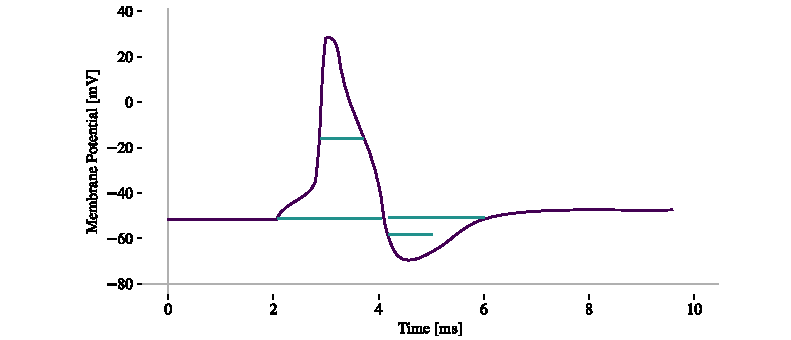
\includegraphics[width=\textwidth]{images/sec_3/action_potential_widths.pdf}
    \caption{}
    \label{fig:2_1_neuron}
\end{figure}

\noindent 
{\bf Peak-to-peak Width:} 
Refered to as type I spike width in the code. 
The width is measured as the time from the minimum potential to the maximum. 
This is a rough measure of the time from the polarization phase to 
the afterhyperpolarization phase. 

The definition can be implemented by measuring the width from
minimum to maximum value, but in cases where the spike is flipped
the definition must also change. 
As such the implementation was done by defining the positive axis along 
the maximum absolute value and calculate the time from 
the maximum value to the preceding minimum value.
\newline


\noindent 
{\bf Half Amplitude Width:} 
Width is measured as the duration the spike is below half amplitude of the 
signal measured from the baseline.
The baseline is commonly set as the value of the start of the signal, 
though this is not always well defined. 
In many cases the start of the signal is chosen trivialy
and if exciting a neuron with a square current the membrane potential will 
rise gradually. 
A more accurate description would be to set the baseline at the firing 
threshold of 
the intracellular spike. 
This is not possible in the case of extracellular spikes,
but here the baseline can simply be set as 0. 
\newline

\noindent 
{\bf Width at Base:} 
Experimentally the width at the baseline is commenly used.
It can be difficult to get a good resolution as spikes are very short
and measured width at baseline gives a longer duration than width at half 
amplitude. 

Calculating width at baseline can pose problems when doing computer simulations
of extracellular spikes as there is no firing threshold. 
If the baseline is set at 0 the duration of spike has a tendency to become 
unnaturally long due to the slight potential created by the charging
of the membrane before firing. 
Experimentally this is not a problem as there is always noise
in the signal. 
When attempting to measure 
the width at baseline for extracellular simulations
the baseline can either be set to some fraction of max amplitude
or set as a constant value. 
Both of these solutions have drawbacks however because 
it makes the threshold be chosen trivially. 
\newline

\noindent 
{\bf Width of afterhyporalization:} 
Certain features of an action potential can be connected
to the 
activation of some ion channels. 
That is why in some cases the duration of the afterhyperpolarization 
desired. 
Two ways to define this duration is the width at base or width at half 
amplitude. 
\newline

%}}} end of 
% Spike Amp. Measurement {{{ %
\section{Spike Amplitude Measurement}
Amplitude is easier to calculate than the width of a spike, 
but there are still different ways to define the amplitude. 
In most cases the amplitude is defined as the distance from a baseline,
in a similar manner as a sinusoid.

% }}} Spike Amp. Measurement %
% Similiarty measure {{{ %
\section{Histogram Similarity Measure}
\label{sec:similarity_measure}
To asses width and amplitude definitions on how well they 
classify interneuron from pyramidal neurons
one needs a way to analyze the resulting data. 
To asses how well a variables can be seperated into groups,
such as the width from either pyramidal neurons or 
interneurons,
is a classification problem. 
Classification is a big field and 
a high quality classification algorithm is beyond the scope of this project. 
If the seperation between two variables are clear and bimodal
there should still be possible to declare that this variable can
be used as a classification parameter. 

If we assume electrodes are placed randomly around a neuron and calculate
the amplitude and width one can create a probability distribution
of that measure. 
This is done by creating a histogram of the samples 
where the height of the bars are equal to the number of samples within 
that bin. 
By normalizing this distribution we get the measured probability distribution
of that variable. 

% TODO: rewrite. 
Comparing histograms is of fundamental importance in patter classification, 
clustering and information retrival problems. 
From this field we can borrow a measure of the difference betweeen histograms. 
This measure is frequently refered to as the histogram distance. 
As histograms can be viewed as points in multidimensional space 
the histogram distance are also commonly refered to as a metric. 

Choosing an aproptiate metric should be fit to the spesific data and results
desired. 
To keep things simple two metrics have been choosen for this project, 
the (ROC AUC) and a simple intersection metric. 

\noindent
{\bf Receiver Operator Characteristic Area under Curve}
Useful binary classifier. 
\begin{figure}[h]
    \begin{center}
        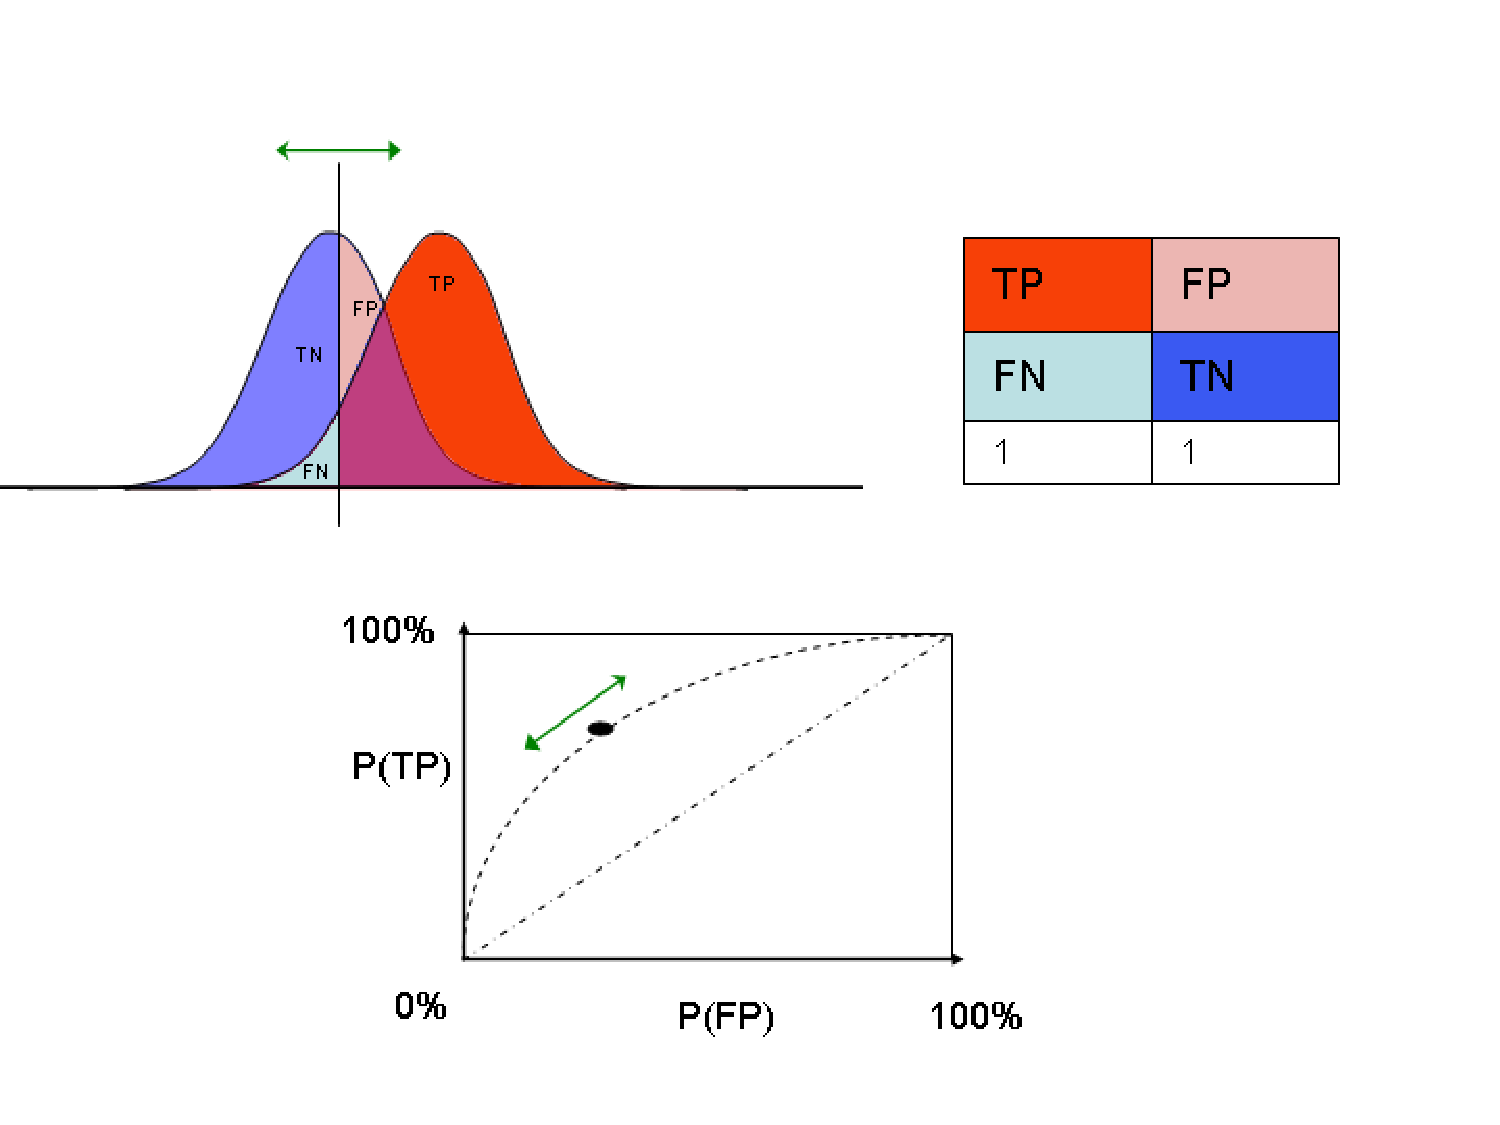
\includegraphics[width=0.5\textwidth]{images/sec_3/roc_curve.pdf}
        \caption{
            ROC curve. 
        }
        \label{fig:3_roc_auc}
    \end{center}
\end{figure}
\newline 

\noindent
{\bf Simple Overlap}
The metric is simply defined as the overlap
of two histograms. 
It can be defined similar to the intersection divided by the union of sets, 
the Jaccard Index. 
One source named this metric the histogram jaccard metric. 

This metric was chosen because ROCAUC is only defined for one
dimenensional data and because of its simplicity.
The metric measures 0 when the two variables share no data in common 
and 1 if compared to itself. 
\newline 

\begin{figure}[h]
    \begin{center}
        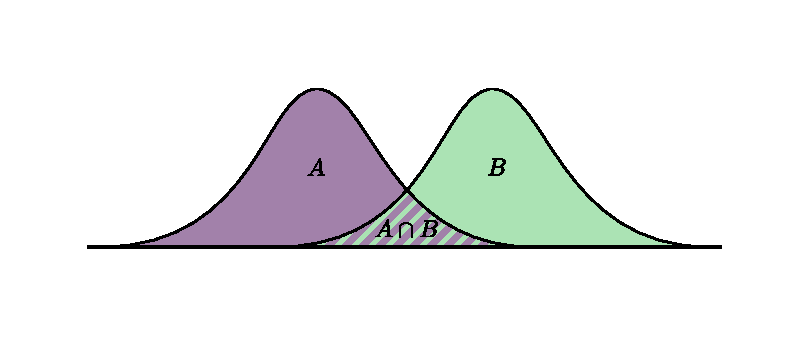
\includegraphics[width=1\textwidth]{images/sec_3/hist_inter.pdf}
        \caption{
            An intersection metric as a way to measure the similarity
            between two distributions.
        }
        \label{fig:3_hist_inter}
    \end{center}
\end{figure}
% }}} Similiarty measure %
% PCA analysis {{{ %
\section{Rotate Cells using PCA}
\label{sec:pca_analysis}
% }}} PCA analysis %
%{{{ Blue Brain
\section{Blue Brain Models}
\label{sec:blue_brain}
Obtaining a reconstruction of the morphology of neurons is an
arduous task which has limitied the number of fully
reconstructed neuron models.

The Human Brain Project Neocortical
Microciruit Collarboration Portal
(\url{bbp.epfl.ch/nmc-portal/welcome},
\textcite{ramaswamy_neocortical_2015})
released mutliple neuron models from the hind limb somatosensory cortex 
of 2-week-old Wistar Han rats.
The models have been classified into both morpholigcal and electrophysical
types with full morphological reconstruction. 

The neuron models are based on the classication criteria set by the Blue Brain 
team.
% there is only 2 classes of pyramidal neurons avaiable in L5, while
% the diversity in interneuron models are much greater.
% The number of available models were based on the variability of 
% neurons depending on their morphological type and 
% electrophysiological response to stimuli.
% As most of the encountered pyramidal neurons had a similar morphological
% structure and response to stimuli the team choose to only recoqnize
% two morphological types and one electrophysiological type, 
% referred to as m-type and e-type.

% Here the models have been simulated with NEURON and LFPy 
% to measure the extracellular potentials. 
% All available models from the L5 area were used.
% To investigate which of the two 
% width definitions is more optimal for differentiating
% interneurons from pyramidal neurons,
% three classes of the most abundant neurons were selected 
% from the blue brain models.
% Two classes of interneurons and one class of pyramidal neurons. 
% There were two classes of pyramidal models available but as the
% one class had identical dendrites it was not analyzed.


% The classes of neurons were Thick Thufted Pyramidal Cell with
% an early bifurcating apical thuft (TTPC2), Large Basket Cell (LBC) and
% Nest Basket Cell (NBC).
% Each of the three class had 5 seperate models where each model
% had different m-type but identical e-type.
% The e-type of TTPC2 class was continuous adapting (cAD), 
% LBC was delayed stuttering (dSTUT) 
% and NBC was continuous non-accommodating (cNAC) 
% (\textcite[463]{markram_reconstruction_2015}).

% Use the models. Write code to capture one action potential. Bursting neurons
% often hav adapting action potential, what to do there. 

%}}} end of Blue Brain
% LFPyUtil{{{ 
\section{LFPyUtil}
% Content {{{ %
\subsection{About}
LFPyUtil is a python package that was created for this project with the purpose
to simplify the simulation pipeline for multiple neurons and creating
an easy to use interface when developing new simulations. 
LFPyUtil extends and uses the package LFPy to accomplish this. 
Simulations can be run in parallel and data from simulations can
automatically be saved and loaded to avoid unnecessary processing time.
LFPyUtil has 9000 lines of code, documentation can be found at
\url{www.documentation.lastis}. 
% TODO
% Some features of LFPyUtil are running simulations in parallel,
% and automatic saving and loading run parameters and data from simulations.

% TODO: Link to where the programming package is saved, pypi, 
% and that it uses python 2 because of NEURON.

% TODO: This paragraph must be made clearer.
LFPy is a Python package created to calculate extracellular potentials.
Another major feature is wrapping the cell model and electrodes
from the NEURON simulation environment into Python objects, such as the 
\verb+LFPy.Cell+ and 
\verb+LFPy.StimIntElectrode+ classes.
This makes working with NEURON more pythonic as 
it can be argued that NEURON is
state-based.
That is, even though the Python interface of NEURON uses objects,
the objects are bound to the state system. 
In practical terms this means that all functions and variables
with NEURON are global static. 

While NEURON has support for paralell processing of single simulations
it does not have 
any inherit support for running multiple independent simulations.
For "embarrasingly parallel" situations like this,
users have had to resort to creating their own methods
to start each simulation independently.
For instance, one solution would be to use a Python script to run other scripts
through the command line, effectivly starting new processes.
In addition there is no function to reset the simulation environment
which can make previous simulations affect later ones.

LFPyUtil uses Python's multiprocessing package to run independent simulations
and thus overcomes some of the shortcomings of NEURON and LFPy.
% }}} Content %
% MWE {{{ %
\subsection{Minimal Working Examples}
These examples show how to create a new custom simulation from
scratch and how to use them with LFPyUtil. 
A basic understanding of object-oriented programming 
and Python is required. 

To run a simulation LFPyUtil must first
have a 
{\verb LFPy.Cell } object
it can use to interact with the model.
The cell object gives access to functions such as 
\verb+Cell.simulate()+
which starts the NEURON simulation.
A template of such a function can be seen in
\cref{code:load_model_simple}. 
A fully working example of such a function can be seen
in the appendix (\cref{code:load_model}).

\begin{listing}[H]
    \caption{load\_model\_simple.py}
    \inputminted[
        frame=lines,
        baselinestretch=0.4,
        fontsize=\footnotesize,
        bgcolor=LightGray,
        linenos
    ]{python}{examples/load_model_simple.py}
    \label{code:load_model_simple}
\end{listing}

LFPyUtil use subclasses of the class
\verb+LFPyUtil.sims.Simulation+.
to organize simulations.
\Cref{code:new_simulation_class_simple} 
shows a very minimal example of such a subclass.
If the functions 
\verb+simulate+, 
\verb+process_data+ and 
\verb+plot+ 
are not overrided, a
\verb+NotImplementedError+ will be raised.

\begin{listing}[H]
    \caption{new\_simulation\_class\_simple.py}
    \inputminted[
        frame=lines,
        baselinestretch=0.4,
        fontsize=\footnotesize,
        bgcolor=LightGray,
        linenos
    ]{python}{examples/new_simulation_class_simple.py}
    \label{code:new_simulation_class_simple}
\end{listing}

The LFPyUtil simulation class has been created 
to reflect four parts of a typical neuron simulation.
(1) Initilization,
(2) simulation/gather data, 
(3) processing data and (4) plotting the data.
These four parts are retained in the initilization
of the object, the \verb+__init__()+ function, 
a simulation function 
\verb+simulate(cell)+, 
a process function 
\verb+process_data()+
and a plotting function 
\verb+plot()+.
Run parameters, plot parameters and data are stored in dictionaries
in the simulation class and the variables are named
\verb+run_param+, 
\verb+plot_param+ and
\verb+data+ respectively.
The LFPyUtil simulation class has additional properties that 
among other things enable saving and loading data and 
naming those files. 
Because of this a new simulation class should inherit
LFPyUtil's simulation class. 

\Cref{code:new_simulation_class} 
defines a simulation class that 
inherits the LFPyUtil simulation class, 
but adds some more functionality.
The function \verb+simulate+
inserts a stimulus electrode and 
applies a current to soma with parameters defined in 
\verb+__init__+. 
The membrane potential is then stored in the 
\verb+data+ dictionary.
The function  
\verb+process_data+
creates a normalized version of the membrane potental
and saves it.
The function \verb+plot+ 
plots the membrane potential.
To exemplify the use of 
\verb+plot_param+, a conditional statement is used
to decide whether or not to plot the normalized version.

\begin{listing}[H]
    \caption{new\_simulation\_class.py}
    \inputminted[
        frame=lines,
        baselinestretch=0.4,
        fontsize=\footnotesize,
        bgcolor=LightGray,
        linenos
    ]{python}{examples/new_simulation_class.py}
    \label{code:new_simulation_class}
\end{listing}

\newpage
The newly created simulation class 
can now be used to run a complete simulation
as seen in 
\cref{code:first_simulation}.

\begin{listing}[H]
    \caption{first\_simulation.py}
    \inputminted[
        frame=lines,
        baselinestretch=0.4,
        fontsize=\footnotesize,
        bgcolor=LightGray,
        linenos
    ]{python}{examples/first_simulation.py}
    \label{code:first_simulation}
\end{listing}

If one attempted to run the simulation function in 
\cref{code:new_simulation_class} 
more than once in the same program,
we would experience that subsequent simulations would be affected by previous
simulations. 
This is because a new electrode will be applied 
once for each call to the simulation function.
With NEURON or LFPy there are no easy way to reset the environment
to prevent this. 
One workaround is to use Python's multiprocessing package
to create multiple independent processes.
Doing this for every simulation will require excessive
amounts of code.
LFPyUtil can simplify this with tools that 
requires less code and are compatible with classes
like the one defined in
\cref{code:new_simulation_class}.


%TODO: Include sentence about how LFPyUtil makes this easier.

The class
\verb+LFPyUtil.Simulator+
accepts one or more objects that inherit
LFPyUtil's simulation 
class and can run them either in serial or paralell
and either in a new independent processes or in the same process. 
\Cref{code:multiple_simulations}
shows how the newly created simulation class can be used with
\verb+LFPyUtil.Simulator+
to run multiple simulations in parallel and in independt processes.

\begin{listing}[H]
    \caption{multiple\_simulations.py}
    \inputminted[
        frame=lines,
        baselinestretch=0.4,
        fontsize=\footnotesize,
        bgcolor=LightGray,
        linenos
    ]{python}{examples/multiple_simulations.py}
    \label{code:multiple_simulations}
\end{listing}

The function 
\verb+Simulator.push+ 
adds the simulation objects to a list.
When the function
\verb+Simulator.simulate()+ 
is ran, the 
\verb+simulate()+ 
function of those objects will be called
in parallel and in independt processes.
The 
\verb+Simulator.plot()+ 
function will call 
\verb+process_data()+ 
and 
\verb+plot(dir_plot)+ 
functions of those objects, and the parameter
\verb+dir_plot+ 
will be created based on the name of the simulation class and
the name of the neuron name.
In this case the plots are stored in the directories 
\verb+./pyramidal_1/plot/custom_sim/+ 
and
\verb+./pyramidal_1/plot/custom_sim_2/+.

The \verb+Simulator+ class utilizes save and load features 
of the simulation class when the 
\verb+Simulator.simulate()+
function is called. 
This makes the dictionaries
\verb+data+
and 
\verb+run_param+
be saved to file.
If 
\verb+Simulator.plot()+
is ran without 
\verb+Simulator.simulate()+
being called first, the program will notice that
the simulations are missing the 
\verb+data+ dictionary.
It will then attempt to load the 
\verb+data+
and 
\verb+run_param+
from file.
After 
\cref{code:multiple_simulations}
has been run once 
line 22 can thus be commented out and the data will be loaded
instead of running the simulation.

LFPyUtil comes with some predefined simulations that have 
been used for results in this article. 
\Cref{code:predefined_simulations}
shows an example of how to use the predefined simulations.

\begin{listing}[H]
    \caption{predefined\_simulations.py}
    \inputminted[
        frame=lines,
        baselinestretch=0.4,
        fontsize=\footnotesize,
        bgcolor=LightGray,
        linenos
    ]{python}{examples/predefined_simulations.py}
    \label{code:predefined_simulations}
\end{listing}

The class 
\verb+MultiSpike+
searches for the input current that will result in 
3 spikes and
then applies that electrode.
It also plots some figures, like the input current and the spikes.
\verb+Intracellular+ 
simulates and plots statistics about some intracellular recordings.
The details of the predefined simulations can be found in 
\cref{sec:simulation_list}
\nameref{sec:simulation_list}.

Note the extra condition,
\verb+False+,
in line 16. 
This tells the simulator that this simulation should not be
run in an independent process. 
When the 
\verb+MultiSpike+
simulation is finished, the electrode it used to generate
3 spikes is still loaded in NEURON.
When the simulation function of 
\verb+Intracellular+ 
runs, the electrode will excite the neuron
and generate 3 spikes.
This feature can be used to link simulations and 
makes the simulations modular.

The previous examples use only one neuron model. 
To be able to run many different models it is usefull to define 
a function such as the one in 
\cref{code:simulator}.

\begin{listing}[H]
    \caption{simulator.py}
    \inputminted[
        frame=lines,
        baselinestretch=0.4,
        fontsize=\footnotesize,
        bgcolor=LightGray,
        linenos
    ]{python}{examples/simulator.py}
    \label{code:simulator}
\end{listing}

To do the same simulation as in
\cref{code:predefined_simulations}, 
one could write:
\begin{listing}[H]
    \caption{run\_simulator.py}
    \inputminted[
        frame=lines,
        baselinestretch=0.4,
        fontsize=\footnotesize,
        bgcolor=LightGray,
        linenos
    ]{python}{examples/run_simulator.py}
    \label{code:run_simulator}
\end{listing}

\Cref{code:multiple_neurons}
runs the two predefined simulations
with two different neuron models.
The class
\verb+LFPyUtil.SimulatorManager+
takes a list of neuron names and passes them to
the
\verb+get_simulator(neuron_name)+
function in 
\cref{code:simulator}. 
The parameter
\verb+neuron_name+
are the elements of the list of 
neuron names.
After running the code once, 
\verb+simm.simulate()+
can be commented out and the simulations will load
data instead of running the simulations.

The final simulation uses three files:
\cref{code:load_model_simple},
\cref{code:simulator} and 
\cref{code:multiple_neurons} and 2 predefined simulation classes.

\begin{listing}[H]
    \caption{multiple\_neurons.py}
    \inputminted[
        frame=lines,
        baselinestretch=0.4,
        fontsize=\footnotesize,
        bgcolor=LightGray,
        linenos
    ]{python}{examples/multiple_neurons.py}
    \label{code:multiple_neurons}
\end{listing}


% }}} MWE %
% }}}
%}}} end of Methods
%{{{ Results
\chapter{Results}
% In figure ?? the spike width from interneurons and pyramidal neurons have been
% plottet seperatly. Neurons in the pyramidal group are the type TTPC1 and TTPC2 
% The groups suggests that interneuron can be seperated from 
% pyramidal neurons depending on their spike shape. 

\vspace{1em} 
\startcontents
\printcontents{}{1}{\setcounter{tocdepth}{3}}

%{{{ Pettersen and Einvoll
\section{Pettersen \& Einevoll (2008) Reproduction}
\begin{wrapfigure}[24]{r}{.5\textwidth}
    \vspace{-20pt}
    \begin{center}
        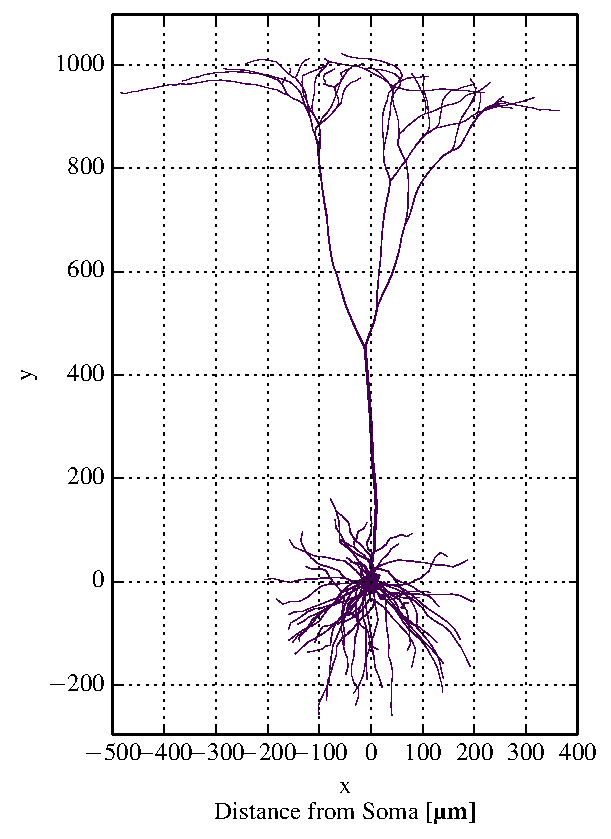
\includegraphics[width=\linewidth]{images/4_1/morph_xy_up.pdf}
        \vspace{-20pt}
        \caption{%
            Morphology of \textcite{mainen_influence_1996} cell. 
            The apical dendrites are located along the y-axis after rotation
            with PCA.}
        \label{fig:4_1_morph}
        \vspace{-10pt}
    \end{center}
\end{wrapfigure}
%
To verify that the simulation environment could be trusted 
some results from 
\textcite{pettersen_amplitude_2008} was replicated.
Spesifically the spike width and amplitude dependency in relation to 
the distance from soma was compared to current results. 

% {{{ Setup%
\subsection{Setup}
\textbf{Model:}
The \textcite{mainen_influence_1996} morphology was used with a passive model, which is 
the same model used in \textcite{pettersen_amplitude_2008}. 
The cell was rotated using PCA (principal component analysis) on the compartment
positions.
This calculates three orthogonal vectors such that 
the positions of the compartments 
has the greatest variance along the first principal component, 
second highest along the second and third most along the third.
The first principal component was made paralell to the y-axis which
puts the apical dendrites along this axis
(\cref{fig:4_1_morph}).
\\

% CS model from Dayan Abott can be found in chapter 6, see fig 6.1 
% in the book.
\begin{figure}[h]
    \begin{center}
        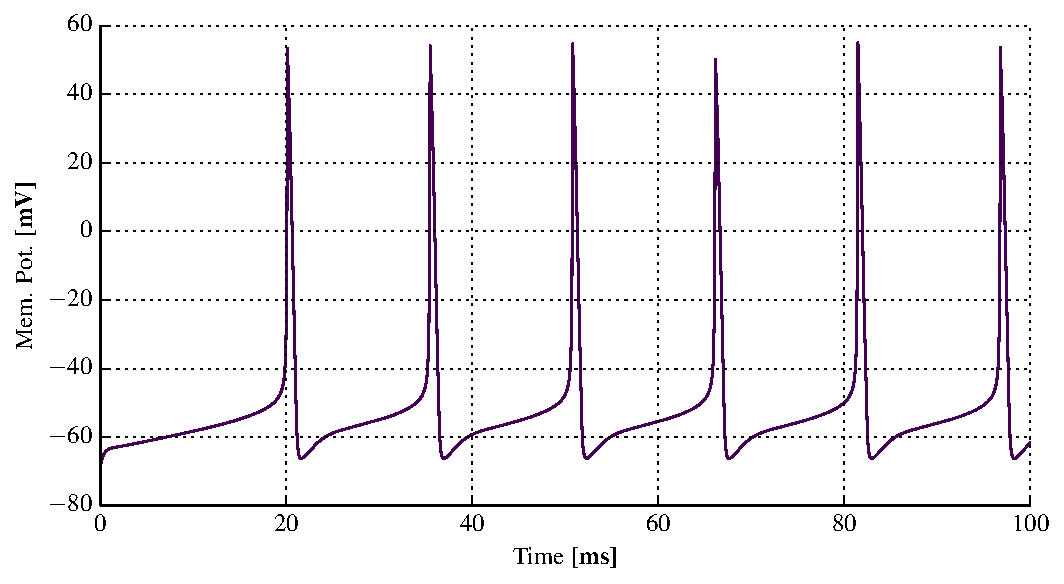
\includegraphics[width=1\textwidth]{images/4_1/cs_ap_original_signal.pdf}
        \caption{
            Simulation of the Connor-Stevens model using parameters from 
            \textcite{dayan_theoretical_2001}. A similar graph is shown in 
            fig. 6.1 (B) in their book.}
        \label{fig:4_1_cs_ap_signal}
    \end{center}
\end{figure}
\noindent
\textbf{Spike Generation:}
To recreate the action potential used in
\textcite{pettersen_amplitude_2008}
a spike was generated using the Connor-Stevens model 
(\textcite{connor_prediction_1971,connor_neural_1977})
using the same parameters as \textcite{dayan_theoretical_2001} and
\textcite{pettersen_amplitude_2008}\@. 
In \cref{fig:4_1_cs_ap_signal} the Connor-Stevens simulation is shown
where the second spike was used for further analysis. 
This spike had an amplitude of \SI{119.49}{\milli\volt} from baseline. 
The baseline was estimated to \SI{-53.26}{\milli\volt} and the
peak at \SI{53.26}{\milli\volt}. 
These values matches \textcite{dayan_theoretical_2001}\@, but not
the spike used in \textcite{pettersen_amplitude_2008} which had an amplitude of 
\SI{83}{\milli\volt} from baseline. 
\textcite{pettersen_amplitude_2008} does not go into further detail about
the creation of the action potential other than stating the action 
potential were similar to \textcite{dayan_theoretical_2001}\@.
The difference might be explained by the fact that action potentials
from pyramidal neurons often peaks at \SI{20}{\milli\volt},
and that this was achived by scaling the original signal from the
Connor-Stevens model.
To compensate for the difference the action potental used in further 
simulations were 
scaled to \SI{83}{\milli\volt} (\cref{fig:4_1_cs_ap_scaled}).

The input current was set to 
\SI{12.6}{\micro\ampere\per\centi\metre\squared}. 
and was very carefully adjusted to make the magnitude spectrum 
(\cref{fig:4_1_fourier})
similar to 
\textcite{pettersen_amplitude_2008}\@ figure 3.
Without adjustment the magnitude spectrum tended to have
a different inital value, from $6$ to \SI{8}{\milli\volt}, and
was not as smooth.
\\

\begin{figure}[h]
    \begin{center}
        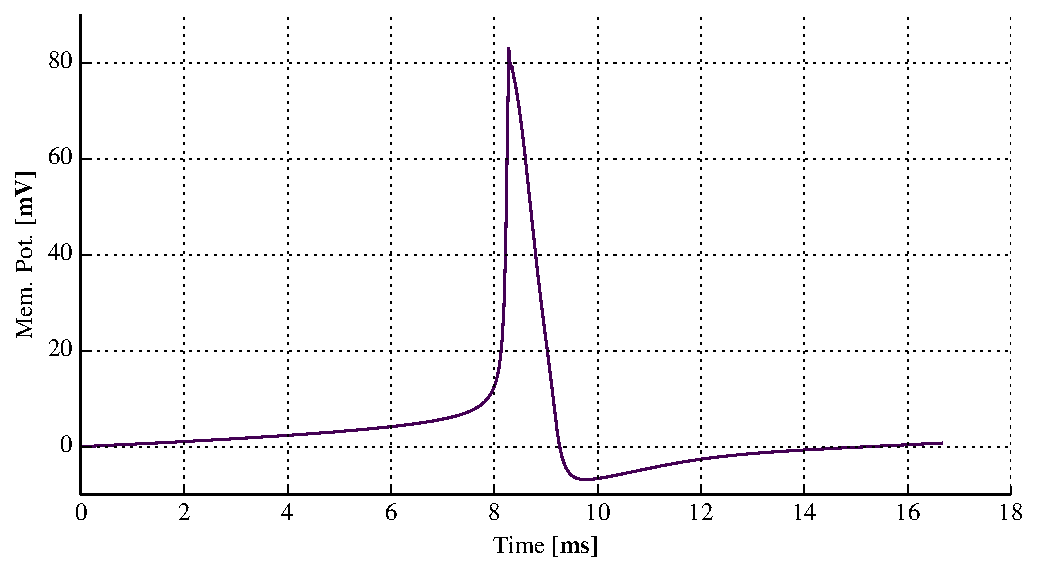
\includegraphics[width=1\textwidth]{images/4_1/cs_ap_scaled.pdf}
        \caption{
            The second spike in \cref{fig:4_1_cs_ap_signal} scaled to 
            \SI{83}{\milli\volt} to match the action potential used in 
            \textcite{pettersen_amplitude_2008}.
            }
        \label{fig:4_1_cs_ap_scaled}
    \end{center}
\end{figure}

\noindent
\textbf{Parameters:}
Parameters for the Neuron simulation were the same as 
\textcite{pettersen_amplitude_2008} and the aforementioned 
action potential was 
used as a boundary
condition in soma.
This was accomplished by 
setting the membrane potential equal to the 
action potential in all
soma sections using the 
{\verb .play }
vector function in Neuron.
This "excites" the neuron even though there are no
ion channels in the model.

Membrane resistance 
$R_m = \SI{30}{\kilo\ohm\per\centi\metre\squared}$, 
membrane capacitance 
$C_m=\SI{1}{\micro\farad\per\centi\metre\squared}$, 
axial resistance 
$R_a = \SI{150}{\ohm\per\centi\metre\squared}$, 
time resolution 
$dt = \SI[exponent-base=2]{e-5}{\milli\second}$. 
The reversal potential was set to zero. 
\\

\begin{wrapfigure}[19]{r}{.5\textwidth}
    \vspace{-20pt}
    \begin{center}
        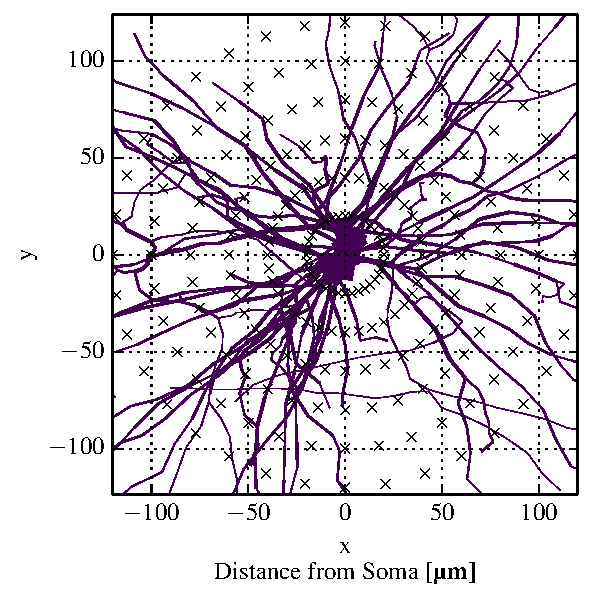
\includegraphics[width=\linewidth]{images/4_1/disc_morph_elec_xz.pdf}
        \vspace{-20pt}
        \caption{%
            Electrode positions placed in a plane around soma perpendicular to
            the axis along the apical dendrites.
            }
        \label{fig:4_1_electrode_pos}
        \vspace{-10pt}
    \end{center}
\end{wrapfigure}
\noindent
\textbf{Electrode Positions:}
Recording sites were placed in the xz-plane at 11 linearly spaced 
positions along 36 lines with equal 
angular spacing (\cref{fig:4_1_electrode_pos}).
\textcite{pettersen_amplitude_2008} states the recording positions
were in the plane perpendicular to the apical dendrites, this is 
ensured by the rotation done with PCA and putting the electrodes in
the xz-plane.
\\


\noindent
\textbf{Spike Width \& Amplitude:}
A baseline was set as the value at the start of the signal. 
Amplitude was calculated as the difference between the maximum value and the
baseline.
The spike width was calculated at as the width at half maximum value. 

At 
$dt = \SI[exponent-base=2]{e-5}{\milli\second}$,
the spike width from the Connor-Steven model was 
\SI{0.5625}{\milli\volt}.
This is similar to the reported spike width from
\textcite{pettersen_amplitude_2008} which was
was \SI{0.55}{\milli\second}.
Because the $dt$ used in their simulations was
$dt = \SI[exponent-base=2]{e-5}{\milli\second} = \SI{0.03125}{\milli\second}$,
their resulting spike width 
must have been rounded to
the nearest \SI{0.05}{\milli\second}.

% }}}  %
% {{{ Results %
\subsection{Results}
The action potental that was used in \textcite{pettersen_amplitude_2008} 
is similar to the one used here.  The amplitude of the fourier transform is displayed in
\cref{fig:4_1_fourier}, which is in close resemblance to the action potential
in fig. $3$ in the paper. 

\begin{figure}[thp]
    \centering
    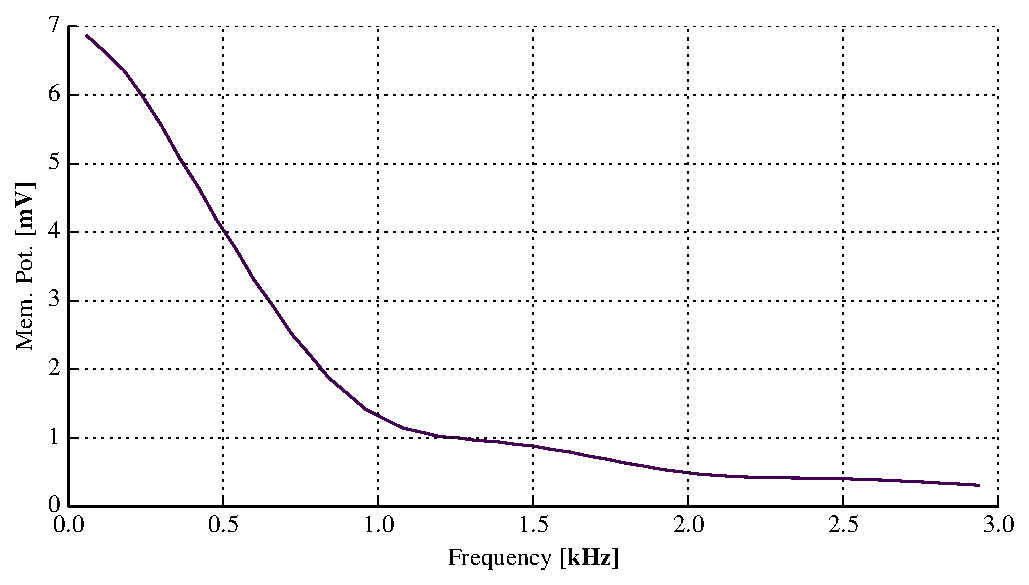
\includegraphics[width=\textwidth]{images/4_1/cs_ap_fourier.pdf}
    \caption{Magnitude specter of simulated somatic membrane potential.}
    \label{fig:4_1_fourier}
\end{figure}

The spike width increases with the distance from soma as seen in 
\cref{fig:4_1_spike_width}. 
These results from
\textcite{pettersen_amplitude_2008}
show an initial spike width of about
\SI{0.5}{\milli\second}
at 
\SI{20}{\micro\metre}
to 
\SI{0.8}{\milli\second}
at 
\SI{120}{\micro\metre}.
Current results are higher than the reported widths
by about 
\SI{0.1}{\milli\second}
at every distance. 
The spike width is defined as width of the negative phase
at $25\%$ of the maximum amplitude. 
If the spike width is adjusted to $35\%$ of the maximum amplitude
the results match nearly perfectly, though the importance
of this is unclear. 

Sudden changes in spike width was experienced with increased distance from
soma. Above $200\mu V$ the
most of the spikes shapes are not well defined. 
This was also reported in \textcite{pettersen_amplitude_2008}\@.

\Cref{fig:4_1_spike_amp} shows the spike amplitude with logarithmic axes.  
The exact results from 
\textcite{pettersen_amplitude_2008}
are not available but 
the approximate value can be seen from their plots and
the exponential decay
$1 / r^n$
was reported
as  $n \sim 2$ at \SI{20}{\micro\metre} and 
$n \sim 2.5$ at \SI{120}{\micro\metre}.
Current results are not identical to those findings
and have an exponent 
of $n = 2$ at \SI{20}{\micro\metre}
and $n = 2.8$ at \SI{120}{\micro\metre}.
The value of the amplitude was about
\SI{350}{\micro\volt} in 
\textcite{pettersen_amplitude_2008}, 
but the current model only gives an amplitude of 
\SI{120}{\micro\volt} 
at 
\SI{20}{\micro\metre}.

\begin{figure}[thp]
\centering
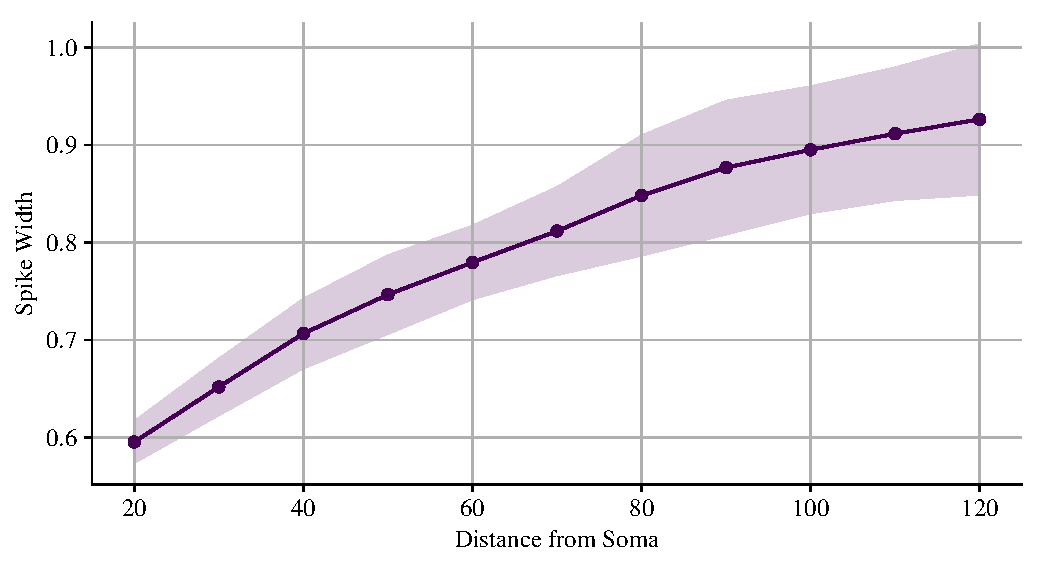
\includegraphics[width=\textwidth]{images/sec_4/disc_spike_width_II.pdf}
\caption{Spike width over distance. Mean +/- 1 std.}
\label{fig:4_1_spike_width}
\end{figure}

\begin{figure}[thp]
    \centering
    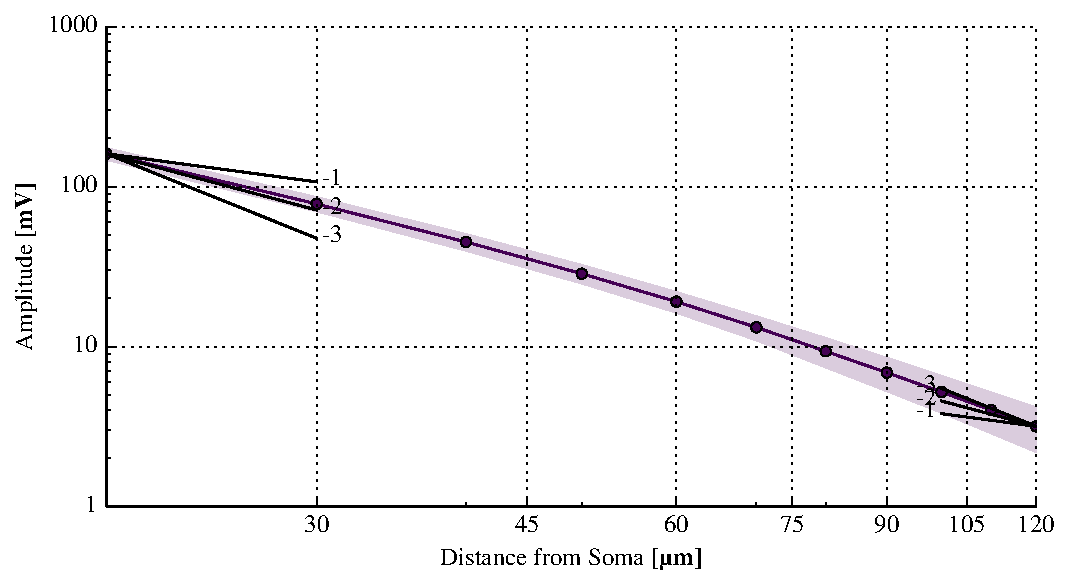
\includegraphics[width=\textwidth]{images/4_1/disc_spike_amps_I_log.pdf}
    \caption{Spike amplitude over distance. Mean +/- 1 std. The power law
    decays $1/r$, $1/r^2$ and $1/r^3$ are shown at the leftmost and rightmost
    data points.}
    \label{fig:4_1_spike_amp}
\end{figure}
% }}}  %
% {{{ Discussion%
% \subsection{Discussion}

% }}}  %
%}}} end of Pettersen and Einvoll
%{{{ Blue brain models. 
\newpage
\section{Blue Brain Simulations}
The number of previous simulations of extracellular action potentials are
few. 
The publicly avaiable models from the Blue Brain
(\cref{sec:blue_brain})
include neuron models with full reconstruction of the morphology. 
The neuron models are ment to cover the whole diversity of neuronal
types encounted in the mouse somatosensory cortex. 
This is one of the first simulations where 
the extracellular action potentials
of a large number of different neuronal types are being compared. 

Spike widht and amplitude are known to be markers 
for pyramidal neurons and interneurons. 

Many different definitions of spike width has been used to differentiate neurons
and it is not clear which spike definitions are better suited for classification.
Here models from the Human Brain Project
has been used to question
if some spike width definition prove better than others for classification.
% In order to investigate the difference in
% spike width and amplitude 
\newline
% Setup {{{ %
\subsection{Setup}
\noindent
\textbf{Models:}
Each simulation uses all available models in the L5
area. 
The pyramidal models consisted of models
from 4 me-types with the morphologies
TTPC1, TTPC2, STPC, and UTPC and the same e-type. 
The interneuron models consisted of the remainding 48 me-types.
Each me-type had 5 models which in total summed to 20
pyramidal models and 240 interneuron models. 

%TODO:
In this interneuron group many of the 
me-types represent only
a small portion of the number of neurons found in L5. 
The findings from 
\textcite{markram_reconstruction_2015} 
suggest
that overall the ratio between pyramidal neurons
and interneurons is around $87\% \pm 1\%$. 
And of those interneurons $50\%$ were classified as 
baskets cells (LBC and NBC).
The interneurons from L5 were seperated into 
9 m-types (morphological) and 10 e-types (electrophysiological)
which gave a total number
of 48 uniquie models.

Each of the 5 models in a me-type 
have a slightly different morphological
shape and/or firing pattern. 
Though the degree of difference is not made clear in the 
model documentation. 

All neuron models were rotated using PCA before simulations were
instigated 
(\cref{sec:pca_analysis}).

The extracellular conductivity was set to 
$\sigma = \SI{0.3}{\ohm\metre}$
based upon data from experimental measurements. 
\newline

\noindent
\textbf{Spike Generation:}
Spikes were created using the simulation class
\nameref{sec:multispike}
(\cref{sec:multispike}). 
For each model 3 spikes were provoked during
a simulation of 
\SI{1000}{\milli\second}
with a square current pulse of equal duration. 

All stimulus electrodes uses the {\verb LFPy.StimIntElectrode } with 
a custom made electrode named ISyn. 
With the default stimulus, 
\verb+IClamp+, 
the sum of the transmembrane 
transmembrane 
currents are equal
to the input current. 
With ISyn the currents are correctly
summed to $0$.
\newline

\noindent
\textbf{Electrode placement:}
% The maximum distance an electrode can pick up the signal from neurons highly depends
% on the quality of the electrode used, 
% but by todays standards the distance can usually be no longer than 
% \SI{100}{\micro\metre}.
In most experiments when electrodes are placed in the brain the distance
from the elcetrode to the neurons are usually unknow. 
The electrodes positions are usually adjusted until they 
pick up a signal from nearby neurons. 
To simulate this type of positioning, the electrodes
were placed at random locations around the soma.

Electrodes were placed using the simulation class
\nameref{sec:sphererand} 
(\cref{sec:sphererand}).
1000 electrodes were placed around each soma within a distance
of 
\SI{60}{\micro\metre}. 
This max distance were chosen because even models with the strongest
extracellular amplitude were no higher than 
\SI{50}{\micro\volt}
at a distance of 
\SI{60}{\micro\metre}. 

As the electrodes were randomly placed in euclidian space 
the number of electrodes per distance $r$ increases as a function
of $r^2$. 
Electrodes closer than 
\SI{15}{\micro\metre}
have been ignored since not all models had
any electrodes within this distance. 

% }}} Setup %
% {{{ Optimal Spike Width%
\newpage
\subsection{Choosing the Optimal Width Definition}
\label{sec:optimal_width_def}
% \begin{wrapfigure}[22]{r}{.5\textwidth}
%     \vspace{-20pt}
%     \begin{center}
%         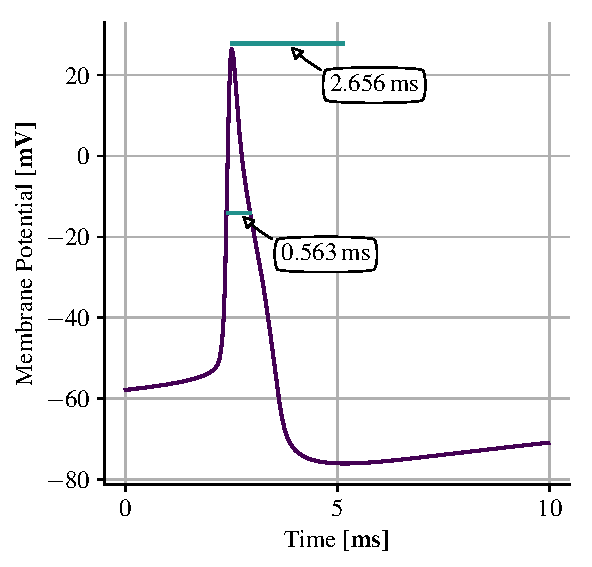
\includegraphics[width=\linewidth]{images/sec_4/widthdef_soma_mem_small.pdf}
%         \vspace{-20pt}
%         \caption{%
%             Two commonly used spike width definitions, 
%             the peak-to-peak spike width
%             (\SI{2.656}{\milli\second})
%             and 
%             the width at half amplitude
%             (\SI{0.563}{\milli\second}),
%             respectively referred to as Type I and Type II in the programs.
%             Measured from the soma from a simulation of a nested basket cell 
%             (model L5\_NBC\_L5\_NBC\_cNAC187\_1).
%             }
%         \label{fig:4_width_def}
%         \vspace{-10pt}
%     \end{center}
% \end{wrapfigure}

\begin{figure}[h]
    \begin{center}
        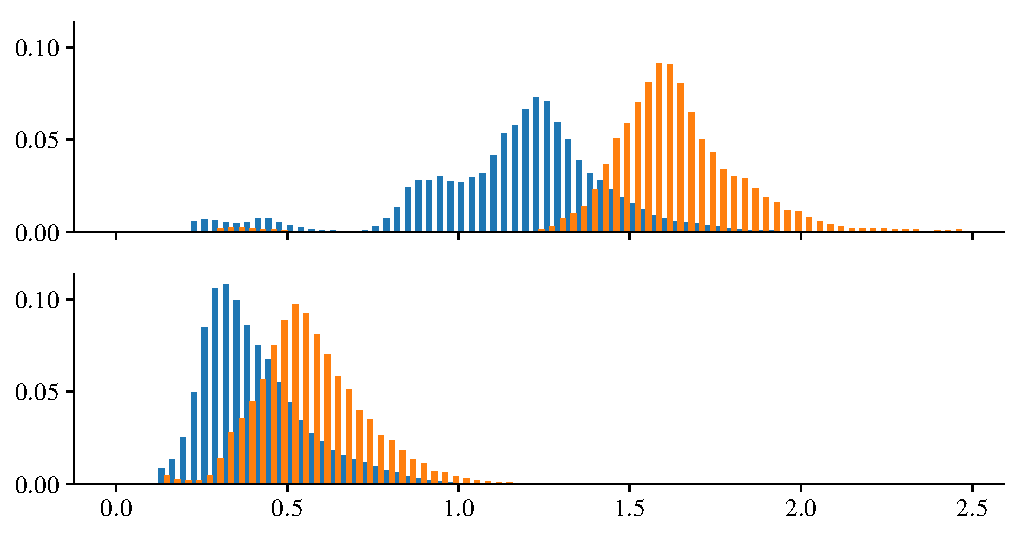
\includegraphics[width=\textwidth]{images/sec_4/int_pyr_width_I_II.pdf}
        \caption{
            Spike widths of all L5 interneuron and pyramidal models from
            the simulations. 
            Top is peak-to-peak spike width; bottom is 
            width at half amplitude.
            Width measurements has been binned by the size of the simulation timestep 
            $dt$.
            Width of the bars are half $dt$.
            The histograms represent a probability distribution of measuring a width
            given a neuronal type. 
        }
        \label{fig:4_width_I_II_histograms}
    \end{center}
\end{figure}

\begin{wrapfigure}[22]{r}{.5\textwidth}
    \vspace{-20pt}
    \begin{center}
        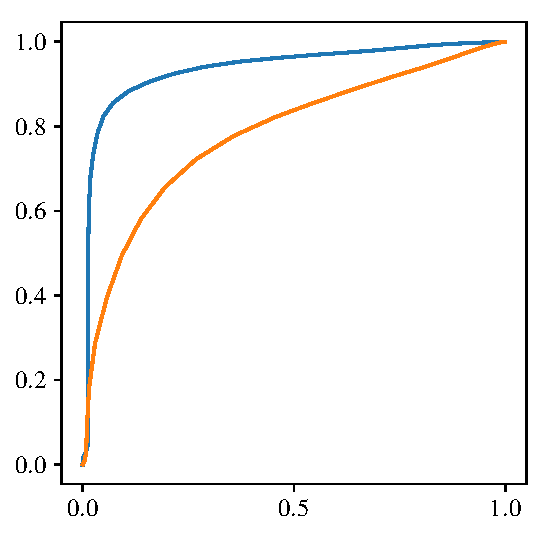
\includegraphics[width=\linewidth]{images/sec_4/roc_curves.pdf}
        \vspace{-20pt}
        \caption{%
            Comparisons between each group of models using ROC curves
            of the width samples of pyramidal neurons and interneurons. 
            Graphs closer to $(0,1)$ indicate a better seperation
            of the models. 
            The peak-to-peak area under curve is $0.94$ while
            area under curve of half-amplitude width is $0.78$.
            }
        \label{fig:4_roc_curves}
        \vspace{-10pt}
    \end{center}
\end{wrapfigure}

Some investigation has previously gone into which features of 
the action potential 
are best suited
for classifying neurons. 
\Textcite{bartho_characterization_2004}
evaluated several spike features and 
concluded that
the spike duration most reliably gave the best seperation between pyramidal neurons and
interneurons. 
Moreover they suggested that the peak-to-peak width definition
of the unfiltered trace reliably gave the better bimodal distributions
than the half-amplitude width. 
Their experiments were carried out in
the somatosensory cortex and prefrontal cortex of both anethesiased
and drug-free mice.
\newline

\noindent
\textbf{Width Distribution:}
A good width definition is recoqnized by having a better
seperation between interneurons
and pyramidal neurons. 
The extracellular spike width was recorded from each of the
electrodes and binned by according to the spike width.
The resulting histogram was then used for the basis
of measuring the seperation between neuron models 
(\cref{fig:4_width_I_II_histograms}).

For both deifinitions the spike width of interneurons are smaller
than the width of pyramidal neurons. 
These findings are in line with previously established research.
%TODO: source.

The histograms represent a probability distribution of
measuring a certain spike width given the neuronal type. 

Little overlap of the neurons models signify
a good ability to seperate the models into two classes. 
It is useful to have a metric to measure the seperation 
between models.
A proper distance metric for histogram data is already 
an important component for some machine learning tasks. 

Though the classification this data is better suited for a
meachine learning algorithm 
it is still useful to have a number on the seperation 
between the neuron models. 
A common measure of the perfomance of a binary classifiers
are ROC curves. 
The area under curve of the ROC, often called the AUC, 
has been used as a measure 
of the accuracy of the classifyer. 
Figure \cref{fig:4_roc_curves}
shows the ROC curves of the two width definitions. 
The AUC was
$0.94$
for the peak-to-peak definition and 
$0.78$
for the half-amplitude 
definition. 
In this case the peak-to-peak definition serves as a better
classification criteria then half-amplitude.
\newline

\noindent
\textbf{Width by Distance from Soma:}

\begin{figure}[h]
    \begin{center}
        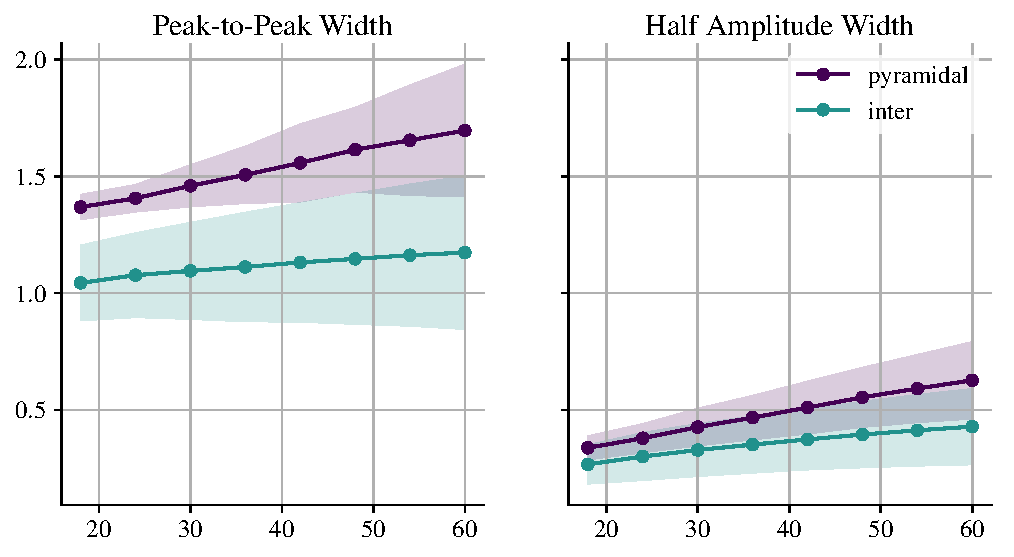
\includegraphics[width=\textwidth]{images/sec_4/int_pyr_widths_dist.pdf}
        \caption{
            Comparison of the spike width by distance from soma using the peak-to-peak
            and the half-amplitude definition.
            Each measurement from the electrodes have been binned into 8 bins
            and the mean and standard deviation was calculated. 
            Half-width width shows a higher overlap at all distances than peak-to-peak
            definition. 
        }
        \label{fig:4_width}
    \end{center}
\end{figure}

The two spike widths were recorded and binned according 
to their distance from soma
(\cref{fig:4_width}).
The lower and upper bounds of each graph is 
$1$ s.t.d.
It is immediately clear that the seperation 
is higher for the peak-to-peak width. 
\newline

\noindent
\textbf{Variance:}
To evaluate the precision of the two width definitions
the coefficient of variation, $c_v$,
was used rather than the variance. 
\begin{align}
    c_v = \frac{\sigma}{\mu}
\end{align}

Because the variance is of similar magnitude for both width definitions, 
the overall greater mean of the peak-to-peak width results in a
lesser $c_v$ at all distances 
(\cref{fig:4_width_snr}).
This suggests that 
the peak-to-peak width
is more accurate than the half-amplitude width. 
The peak-to-peak width is also generally has longer 
durations which makes it easier to measure for real electrodes. 

% An example is the $\sigma$ at 
% \SI{50}{\micro\metre}
% for the group "All Inter" from \cref{fig:4_2_width}.
% For Type I 
% $\sigma = \SI{0.25}{\milli\second}$ 
% and 
% $\mu = \SI{1.1}{\milli\second}$, 
% while for Type II 
% $\sigma = \SI{0.15}{\milli\second}$ 
% and 
% $\mu = \SI{0.3}{\milli\second}$. 
% The variance is lower for Type II but is also
% almost $50\%$ of the mean value. 
% The variance from Type I is higher, but is only about 
% $25\%$ of the mean value, 
% which makes Type I more accurate than Type II.


\begin{figure}[h]
    \begin{center}
        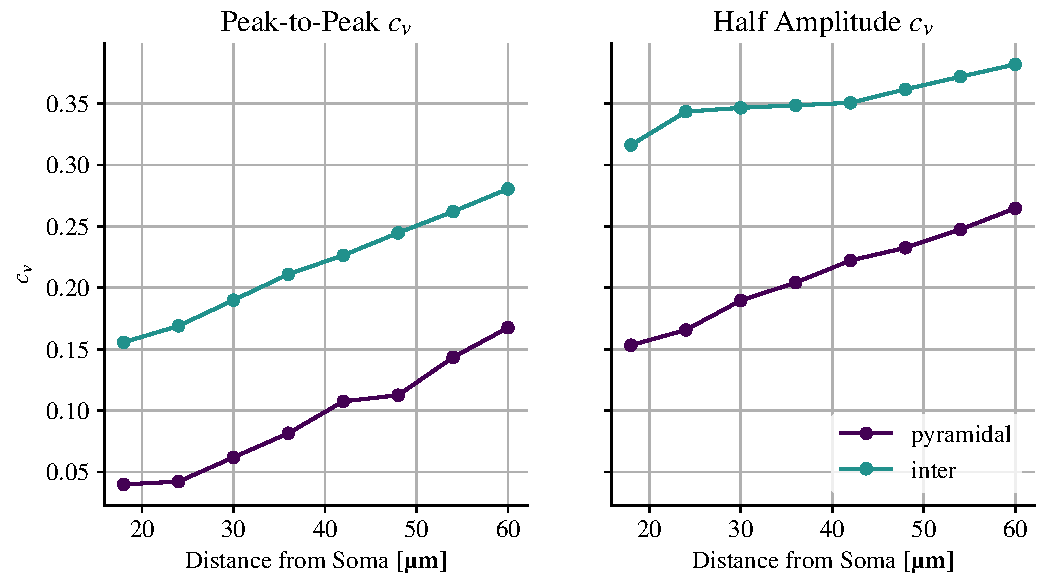
\includegraphics[width=\textwidth]{images/sec_4/int_pyr_widths_snr.pdf}
        \caption{
            Coefficient of variation, $c_v$, calculated from \cref{fig:4_width}.
            A lower coefficient of variation entail a more precise measurement.
            $c_v$ is lower at all distances for the peak-to-peak definition compared
            to the hal-amplitude definitions for both
            pyramidal neurons and interneurons. 
        }
        \label{fig:4_width_snr}
    \end{center}
\end{figure}



\noindent
% }}}  %
% {{{  Optimal Amplitude Definition%
\newpage
\subsection{Choosing the Optimal Amplitude Definition}
The two amplitude definitions investigated are
the amplitude from baseline and 
the peak-to-peak amplitude definition.

% Interneurons and pyramidal neurons cannot reliably be classified 
% based on amplitude alone. 
\Cref{fig:4_amp_distance} shows the amplitude over distance from soma. 
Though there is a clear seperation between pyramidal neurons and interneurons
at a given distance, the distance is usually unknown during experiments. 
The resulting histogram (result not shown) when ignoring distance does not show a clear
biomodal distribution and as such is not suited as a
classification parameter alone. 

\begin{figure}[h]
    \begin{center}
        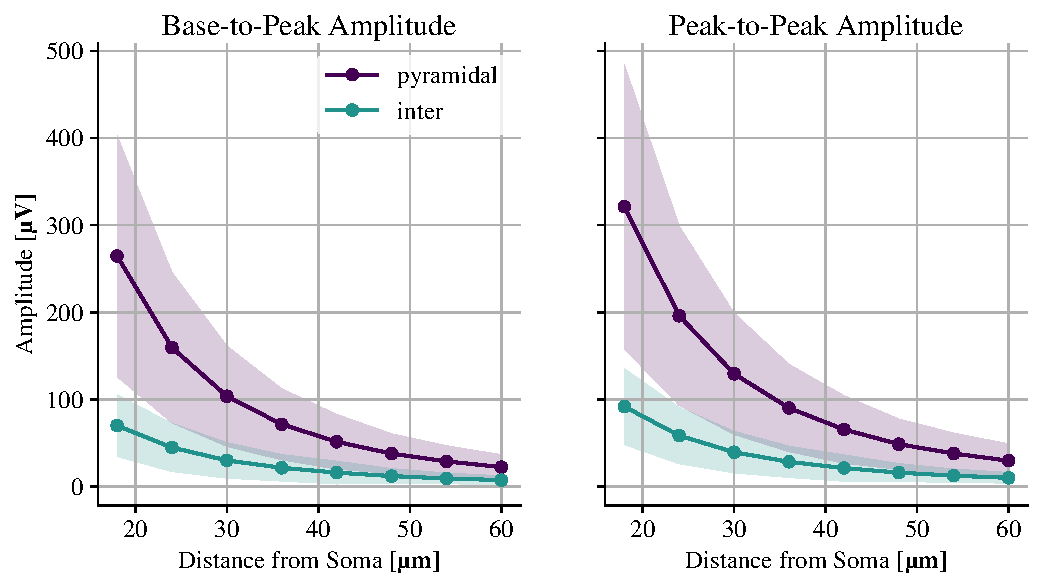
\includegraphics[width=\textwidth]{images/sec_4/int_pyr_amps_dist.pdf}
        \caption{
            Amplitude measurements by distance from soma. 
            Analysis is done identical to spike width from soma (\cref{fig:4_width}). 
            Based on seperation between neuron types
            neither definition shows a clear advantage over the other
            as the overlaps are similar. 
        }
        \label{fig:4_amp_distance}
    \end{center}
\end{figure}

There seems not to be a clear distinction of which amplitude definition is better. 
As with the width definition we can calculate the coefficient of variation 
to compare the accuracy of the definitions. 
The coefficient of variation (results not shown) 
is lower for the peak-to-peak width definition at all distances.  
This can be attributed to that the variance for both definitions are similar 
while the mean value of peak-to-peak amplitude is always higher. 

% }}}  %
% {{{ Classifying Neurons%
\newpage
\subsection{Combining Spike Width and Amplitude}
\begin{figure}[h]
    \begin{center}
        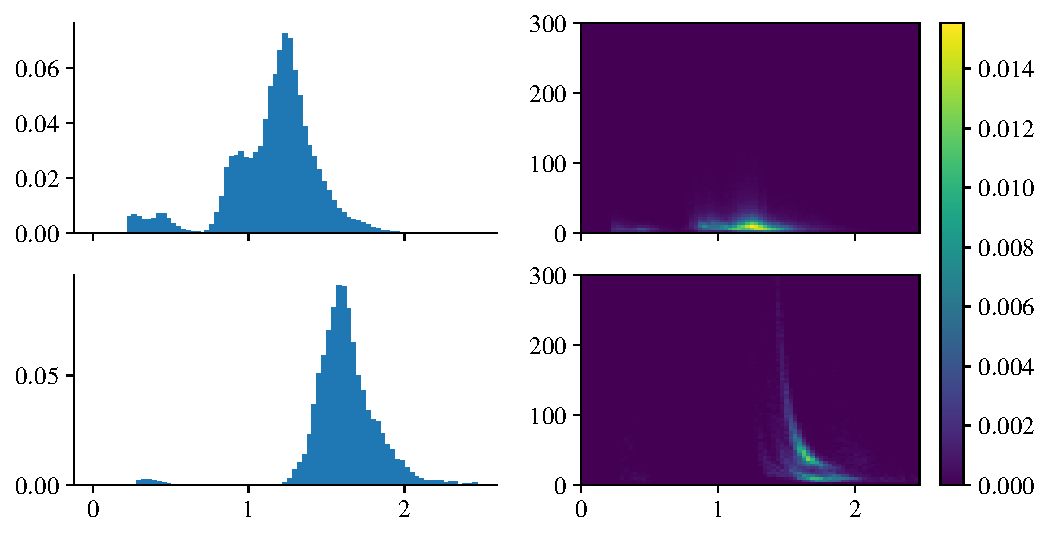
\includegraphics[width=\linewidth]{images/sec_4/int_pyr_hist.pdf}
        \caption{Spike width and amplitude histograms of interneurons
        and pyramidal neurons. 
        The overlap of these two distributions
        is $5.10\%$. 
        The overlap of the spike width distributions
        alone is $12.15\%$. 
        }
        \label{fig:4_int_pyr_hist}
    \end{center}
\end{figure}

As long spike widths from interneurons accompany 
low amplitudes and short spike widths from pyramidal neurons
accompany high amplitudes it is reasonable to conclude that
the amplitude could be used as an addition parameter for classification. 
From this point on the peak-to-peak width and amplitude 
definitions will be used. 

The spike width and amplitude
can be combined into
2d histograms as seen in the right column of
figure \cref{fig:4_int_pyr_hist}. 
The left column shows the histogram only based on spike width.
The histograms are made from the spike width and amplitude
data from all pyramidal (20) and interneuron models (250) from L5.

When combining spike amplitude and spike width it is no longer
possible to apply the AUC similarity metric as was done in 
% Optimal Width Definition
\nameref{sec:optimal_width_def}
(\cref{sec:optimal_width_def}).
To compare pyramidal neurons against interneurons
the histograms were compared using a similarity metric 
defined as the histogram intersection divided by the union 
\nameref{sec:similarity_measure}
(\cref{sec:similarity_measure}).
This metric can be interpreted as the overlap between the two histograms
and is a valid metric for both 1d and 2d histograms.

A considerable difference was seen when comparing the overlap
between the histograms. 
When only using spike width the overlap between interneurons
and pyramidal neurons was $12.15\%$.
In the case of spike width and amplitude the overlap
was $5.10\%$.
This suggests that using spike amplitude as an additional 
parameter for classification will give a more accurate result. 
\begin{figure}[h]
    \begin{center}
        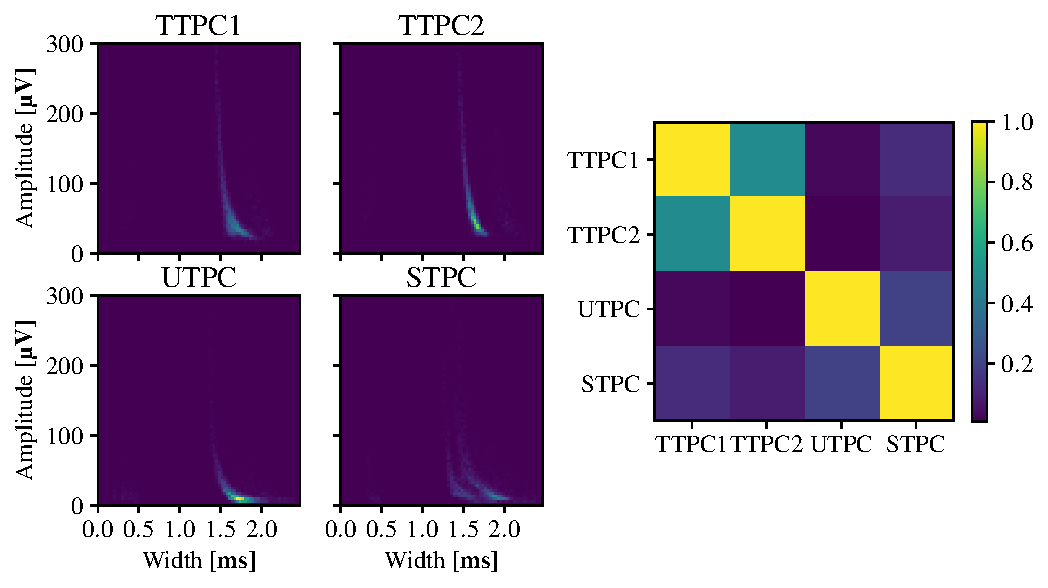
\includegraphics[width=\linewidth]{images/sec_4/pyr_overlap.pdf}
        \caption{
            Comparison of the pyramidal types. 
            Each group is a differnt
            morphological type classified but share the 
            electrophysiological type. 
            Right side shows the overlap of each histogram. 
            The thick thufted morphological types (TTPC1, TTPC2)
            have more in commen than the untufted (UTPC) 
            and slender-tufted (STPC). 
            This suggests that
            pyramidal cells can be split into subclasses using spike width
            and amplitude alone. 
        }
        \label{fig:4_pyr_overlap}
    \end{center}
\end{figure}
The spike width and amp. 2d histogram of the pyramidal models
has a multimodal distribution that could suggest this group could
be split into subclasses (\cref{fig:4_int_pyr_hist}).
This could be a result of
a low diversity among the pyramidal models as 
the pyramidal data is based on 20 models versus 240
interneuron models. 
Though there is a much higher number of interneuron models,
the number of models were based on the diversity of neurons encountered
in the mouse somatosensory cortex. 
If the diversity in the pyramidal models correctly represent the
diversity in the mouse brain it will be possible to classify some
subclasses of pyramidal neurons based only on spike width and
amplitude.

\Cref{fig:4_pyr_overlap} shows the histograms of the 
different classes of pyramidal neurons 
where each class has 5 models.
Each of these classes are me-types but also represents the
morphological class, the m-type, as the pyramidal neurons only have one 
e-type. 
Since the firing patterns are similar
the difference of the histograms
show that the morphology has a big impact on the extracellular spikes. 
% Each pyramidal models tends to have a "hockey stick" shaped 
% distribution. 


\Cref{fig:4_pyr_overlap} also shows the overlap between
each of the classes.
The two groups TTPC1 and TTPC2 has a high overlap of $50\%$
and as such they cannot easily be distingushed from another. 
The group UTPC has little overlap with both TTPC1 and TTPC2, but
overlaps STPC with $30\%$. 
This suggests that the pyramidal cells can be distinguished from
each other in at least 2 groups. 
Furthermore the main reason they can be seperated from each other 
is their morphology. 

The interneurons does not show an as easily distinguishable
histogram. 
%}}}
% Filterig effects {{{ %
\newpage
\subsection{Effect of Filtering}
As filtering is a common manipulation of the signal
to remove noise
it is interesting to see if the separation between interneurons
and pyramidal neurons persist when the signals are filtered. 
\Cref{fig:4_int_pyr_hist_filt} shows the same as 
\cref{fig:4_int_pyr_hist} but with the signals
filtered with a bandpass butterworth filter between 
\SI{300}{\hertz}
and 
\SI{6.7}{\kilo\hertz}.
These values were chosen as they are reported as common values for 
bandpassfiltering. 
\begin{figure}[h]
    \begin{center}
        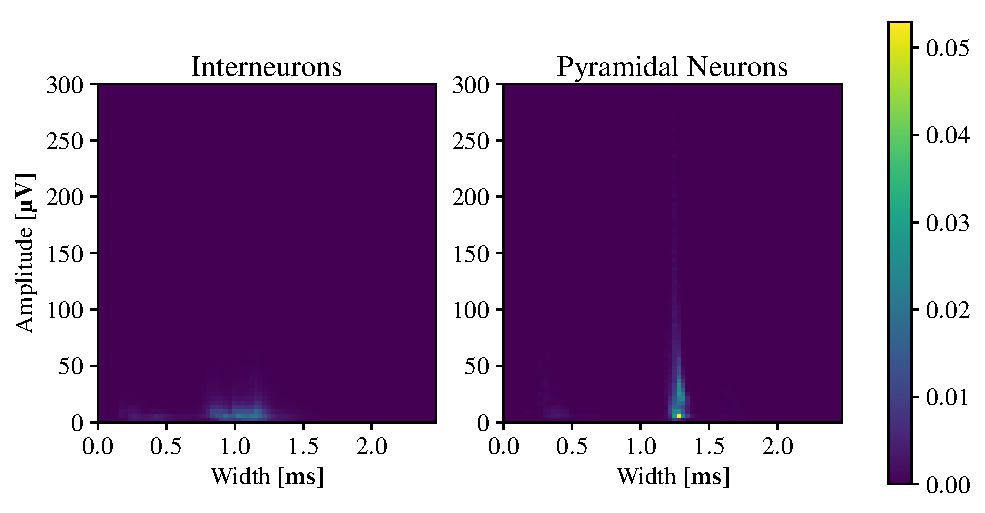
\includegraphics[width=\linewidth]{images/sec_4/int_pyr_hist_filt.pdf}
        \caption{
            Amplitude and width histograms using filtered signals. 
            The shape of the histograms change drasticially compared to
            \cref{fig:4_int_pyr_hist}, though a seperation between 
            interneurons and pyramidal neurons can still be observed. 
        }
        \label{fig:4_int_pyr_hist_filt}
    \end{center}
\end{figure}

Though the histograms have changed drastically, 
the distance metric shows that the models can be seperated 
from each other. 
The overlap in the filtered amplitude width histograms 
are $9.90\%$, an increase from the unfiltered signal that was 
$5.10\%$. 

In the filtered data the different 
pyramidal models are closer together than 
the unfiltered data, 
though they still retain the seperation between them similar as before
(\cref{fig:4_pyr_overlap_filt}).

\begin{figure}[h]
    \begin{center}
        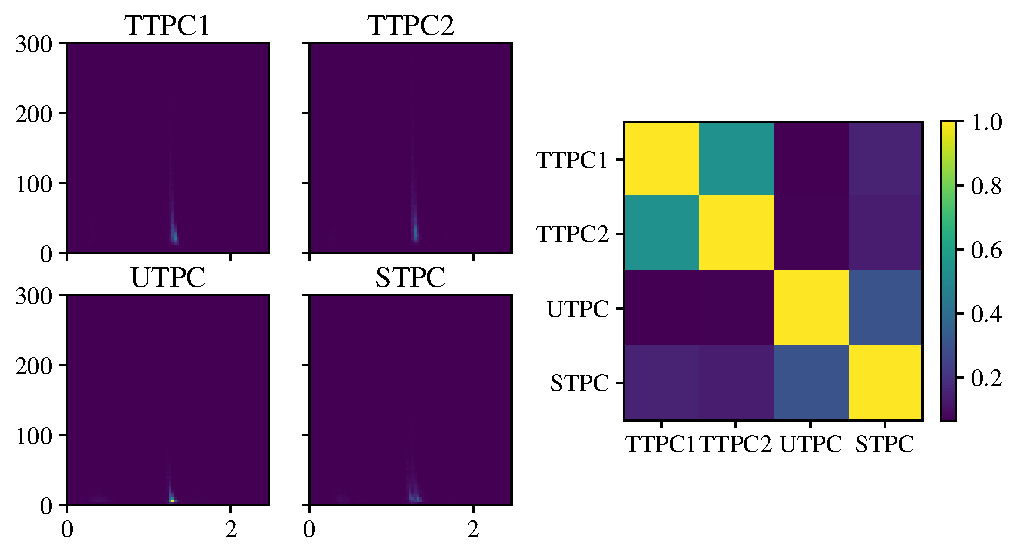
\includegraphics[width=\linewidth]{images/sec_4/pyr_overlap_filt.pdf}
        \caption{
            Comparisong of the individual pyramidal types using the filtered signals.
            Overlap between the histograms are still maintained.
        }
        \label{fig:4_pyr_overlap_filt}
    \end{center}
\end{figure}

% }}} Filterig effects %
% Comparing results {{{ %
\newpage
\subsection{Comparing Results}
Results have been compared to some online sources and a number of articles. 
% The free variables in current simulations are
% the extracellular conductivity and other options to LFPy. 

\noindent
{\bf Neuroelectro:}
The page 
\textcite{_neuroelectro_????}
(\url{http://neuroelectro.org/ephys_prop/23/})
has a collection electrophysiological data 
from a large number of published articles.  
They store data about several features such as spike width, resting potential, 
memrbane time constants 
and other spike data. 
The data is only intracellular measurements
though it gives an insight in the variance of the 
action potentials in the literature. 
The duration of the intracellular action potential is significant 
because it 
heavily effects the extracellular action potential. %TODO: Source

The closest set of data in NeuroElectro 
to the somatosensory cortex is 
neocortex layer 5-6 pyramidal cells. 
The half-amplitude width of these cells were
\SI[separate-uncertainty = true]{1.2 \pm 0.53}{\milli\second}.
This is a very large variance as the 
as the intracellular spike widths for the simulations 
were
\SI[separate-uncertainty = true]{0.70 \pm 0.10}{\milli\second}.
The sources of this variation is hard to approximate. 
It is likely due to a mixture of reasons including
different species of animals, measuring equipment, 
preperation procedures, different brain areas, etc. 
This large variance in spike widths suggests that
comparing data must be done in very similar conditions
as the models are based on. 
\newline

\noindent
{\bf Anastassiou et. al:}
To further compare results 
the models were used to replicate 
some results from the paper
\textcite{anastassiou_cell_2015}.
The focus of this article was 
comparing extracelluar measurements to internal measurements
and the brain area investigated was also the somatosensory cortex. 

They measured the extracellular and intracellular action potential
and looked at how the shape changes as the firing rate of the neuron 
increases. 
It has been reported that the spike width of neurons
increase as the firing rate increases. 

The article also gives an estimate of the extracellular conductivity
which was estimated by fitting the spike amplitude data to the 
function of the potential of a point source. 
$V_e = \frac{I}{\sigma} \frac{1}{4 \pi r}$. 
The values given for the conductivity $\sigma$ in L5 was 
\SI[separate-uncertainty = true]{0.41 \pm 0.24}{\per\ohm\per\metre}.
The high uncertainty was attributed to the estimation of 
the membrane capacity $C$.

\noindent
{\bf \Textcite{bartho_characterization_2004}:}
spike widths  = 0.43 +- 0.27 ms than that of the
putative pyramidal cells 0.86 +- 0.17 ms.
\newline

% }}} Comparing results %
%}}} end of Results
%}}}
%{{{ Discussion
\chapter{Discussion}

% TODO: Fill
Spike Width and Spike Amplitude:
It has been seen that of the spike width definitions investigated here, 
one type of spike width definition is overall
better suited to classify this set of neurons. 
This has also been seen in the literature. 
A similar investigation was done using the spike amplitude and of the
definitions investigated here the peak-to-peak amplitude gave the best
seperation between interneuron and pyramidal neurons. 

Classification:
It has been previously shown that using only spike width as 
a way to classify neurons is not the best. 
Several papers have stated that other methods can be used to give 
a clearer distinction, such as considering the interspike interval. 
Also one group looked at the spike width from axons which gave a short 
durtion. 

Using a simple measure of the similarity between populations
neuron models it can be clearly stated that interneurons can be seperated
from pyramidal neurons. 
Excitatory interneurons cannot be clearly distinguished from the rest of the
interneurons. 
Using machine learning algorithms it might be possible to divide these
into even small groups, how can I show this?
Neurons could probably be seperated into smaller groups based on
spike width and spike amplitude. 

% TODO: Fill
LFPyUtil: 
LFPyUtil is a useful tool that can be used to easily gather
new data when new models arrive. 
As long as a model has the mechanics defined with NEURON and has
a morphology the same simulations and data as seen here can be ran 
and extraced.

% TODO: Fill
The models did now show the expected variance with firing frequency. 
% Article anastassiou is consistent with Nature review, spike shape increases with 
% frequency. 
% This is not the case the models from Blue Brain.

% TODO: Fill
Comparisons with other data:
several articles was investigated to compare current data with.
There is a large variance in the literature of spike widths and amplitude. 
All in all the data fall within the variance of the investigated articles. 
The number range between this and that.


Sources of variation:

% Results are based on spike width and amplitude.
% The basis for all spike shapes are the types and concentrations of
% ion channels.
% This is the central factor that decides if the neuron has short or long action potentials.
% A number things has been observed that can change spike spike width.
% Factors that change action potentials width:
% * Firing frequency.
% * Input current. Higher current gives higher frequency.
% * Number of previous spikes.
% * Bursting behavior.
% * Backproagating action potentials.

% % What are the results, what do you want to show.
% % The grand wish, have a catalogue of all spikes in the brain.
% When plotting spike amplitude over spike width will neurons look different.

% Results: Spike width alone is often used for classifying neurons.
% They often have a bimodal distribution. 
% This is the first time many simulations have been done of the extracellular
% potential.
% Previous research have only used a few models.
% With LFPy and LFPyUtil it will be easy to adapt new models to calculate extracellular potential.

% The spike widths does not show dependency on the firing frequency or spike number.
% Some neurons show this feature and this should do it too.

% Results:
% * Which width and amp definition is most suitable for differention.
% * Classify neurons based on spike width and amplitude.
%     * Compare to other data. 
%     Hard to varify model,
%     values from experiments are vary a lot. 
%     Models were based on result from their recordings. 
%     Cannot see adaption with frequency of any kind.
%     * Is experimental distribution shape similar to mine, if so
%     that is a good result.
% * Development of LFPyUtil. Future neuron models can be adapted for 
% extracellular simulations if they include
% a morphology.

%}}} end of Discussion
% % Appendix {{{ %
\begin{appendices}
\chapter{Appendix}
\startcontents
\printcontents{}{1}{\setcounter{tocdepth}{3}}
% \begin{listing}[H]
%     \caption{load\_model.py - A function to load a Cell object.}
% \begin{mdframed}
    % \inputminted[
    %     breaklines=true,
    %     frame=lines,
    %     baselinestretch=0.4,
    %     fontsize=\footnotesize,
    %     bgcolor=LightGray,
    %     linenos
    % ]{python}{examples/load_model.py}
    % \label{code:load_model}
% \end{listing}
% \end{mdframed}
% Frequently used functions {{{ %
\section{Frequently Used Functions}
\label{sec:frequent_functions}
The simulations use the same functions for 
detecting spikes, 
calculating spike
width and amplitude. 
These functions are used frequently and 
their full implementation is included here. 
The functions are located in the module 
\verb+LFPyutil.data_extraction+.
Other helper functions are also included in this module.
\newline
% \begin{listing}[H]
%     \label{code:width_type_I}
%     \begin{minted}
%     [
%         frame=lines,
%         baselinestretch=0.4,
%         fontsize=\footnotesize,
%         bgcolor=LightGray,
%         linenos
%     ]
%     {python}
%     \end{minted}
% \end{listing}

\noindent
\textbf{Peak-to-Peak Spike Width:}
Spike width is calculated from the absolute maximum value to
the follow opposite minimal value. 
If the absolute value of the minimum is higher than the maximum
value the signal will be flipped. 
The function receives a matrix of spikes, 
where each row is the values of the potential
over time. 
The returned values are an array of spike times
and a matrix with the spike traces. 
The shape of the spike trace matrix is
equal to the input matrix and allows easy plotting. 
\newline

\begin{listing}[H]
    \label{code:width_type_I}
    \begin{minted}
    [
        frame=lines,
        baselinestretch=0.4,
        fontsize=\footnotesize,
        bgcolor=LightGray,
        linenos
    ]
    {python}
def find_wave_width_type_I(matrix, dt=1):
    """
    Wave width defined as time from minimum to maximum.
    """

    matrix = np.array(matrix)
    if len(matrix.shape) == 1:
        matrix = np.reshape(matrix, (1, -1))
    widths = np.zeros(matrix.shape[0])
    trace = np.empty(matrix.shape)
    trace[:] = np.NAN
    for row in xrange(matrix.shape[0]):
        signal = matrix[row].copy()
        offset = signal[0]
        signal -= offset
        # Assume that maximum abs. value is the "spiking" direction.
        if signal.max() < -signal.min():
            signal = -signal
        idx_1 = np.argmax(signal)
        idx_2 = idx_1 + np.argmin(signal[idx_1:])
        widths[row] = idx_2 - idx_1
        trace[row, idx_1:idx_2] = matrix[row, idx_1:].max() * 1.05
    return widths * dt, trace
    \end{minted}
\end{listing}

\noindent
\textbf{Spike Width at Threshold:}
Spike width is calculated a threshold of maximum value, 
with a default value of $0.5$. 
The argument \verb+amp_option+
specifies if which side is considered the spiking direction. 
It can either be 
\verb+'neg'+,
\verb+'pos'+ or
\verb+'both'+. 
In the case of 
\verb+'both'+ 
the maximum value will be considered the spiking direction, 
evaluated for each spike. 
Other input and output variables
are the same as 
peak-to-peak spike width.
\newline

\begin{listing}[H]
    \label{code:width_type_II}
    \begin{minted}
    [
        frame=lines,
        baselinestretch=0.4,
        fontsize=\footnotesize,
        bgcolor=LightGray,
        linenos
    ]
    {python}
def find_wave_width_type_II(matrix, threshold=0.5, dt=1, amp_option='both'):
    """
    Compute wave width at some fraction of max amplitude. Counts the number
    of indices above threshold and multiplies by **dt**. 
    """
    matrix = np.array(matrix)
    if len(matrix.shape) == 1:
        matrix = np.reshape(matrix, (1, -1))
    widths = np.zeros(matrix.shape[0])
    trace = np.empty(matrix.shape)
    trace[:] = np.NAN
    for row in xrange(matrix.shape[0]):
        signal = matrix[row].copy()
        signal -= signal[0]
        # Flip the signal if the negative side should be used.
        if amp_option == 'neg':
            signal = -signal
        elif amp_option == 'both' and signal.max() < -signal.min():
            signal = -signal
        thresh_abs = signal.max() * np.fabs(threshold)
        signal_bool = signal > thresh_abs
        signal_index = np.where(signal_bool)[0]
        widths[row] = np.sum(signal_bool)
        trace[row, signal_index] = matrix[row, signal_index[-1]]
    return widths * dt, trace
    \end{minted}
\end{listing}

\noindent
\textbf{Base-to-Peak Amplitude:}
Amplitude defined as the difference between 
the maximum value and baseline. 
Baseline simply set at the start of the signal. 
Inputs a matrix of spike signals, identical to 
the previous spike width functions.
\newline

\begin{listing}[H]
    \label{code:amp_type_I}
    \begin{minted}
    [
        frame=lines,
        baselinestretch=0.4,
        fontsize=\footnotesize,
        bgcolor=LightGray,
        linenos
    ]
    {python}
def find_amplitude_type_I(matrix, amp_option='both'):
    """
    Finds the amplitude of signals defined as the difference from the 
    maximum value to the start of the signal. 
    """

    matrix = np.array(matrix)
    if matrix.ndim == 1:
        matrix = matrix.reshape([1, -1])
    amp_low = np.zeros(matrix.shape[0])
    if amp_option == 'both' or amp_option == 'neg':
        for row in xrange(matrix.shape[0]):
            amp_low[row] = np.abs(np.min(matrix[row] - matrix[row,0]))
    amp_high = np.zeros(matrix.shape[0])
    if amp_option == 'both' or amp_option == 'pos':
        for row in xrange(matrix.shape[0]):
            amp_high[row] = np.abs(np.max(matrix[row] - matrix[row,0]))
    amp = np.maximum(amp_low, amp_high)
    return amp
    \end{minted}
\end{listing}

\noindent
\textbf{Peak-to-Peak Amplitude:}
Amplitude defined as the duration from maximum value to 
the follow minimal value. 
The maximum value is considered the spiking direction.
Inputs and outputs the same as the previous functions. 
\newline

\begin{listing}[H]
    \label{code:amp_type_II}
    \begin{minted}
    [
        frame=lines,
        baselinestretch=0.4,
        fontsize=\footnotesize,
        bgcolor=LightGray,
        linenos
    ]
    {python}
def find_amplitude_type_II(matrix):
    """
    Finds the amplitude of signals from minimum to maximum.
    """
    matrix = np.array(matrix)
    if matrix.ndim == 1:
        matrix = matrix.reshape([1, -1])
    amps = np.zeros(matrix.shape[0])
    for row in xrange(matrix.shape[0]):
        signal = matrix[row]
        offset = signal[0]
        signal -= offset

        amp_1 = signal.max()
        amp_2 = signal.min()
        amps[row] = np.fabs(amp_2 - amp_1)
    return amps
    \end{minted}
\end{listing}

\noindent
\textbf{Extract Spikes:}
For each spike found in a signal, this function
cuts out an area around the spikes and returns each of 
them in a row in the returned matrix. 
The function was created so
the returned matrix can be inputed to any of the previous functions. 

\verb+t_vec+ must be a 1d array of the simulation time in milli seconds. 
Spikes will be extracted from the 1d array \verb+v_vec+, 
that could for instance be from a single electrode or a membrane potential. 

\verb+pre_dur+
and 
\verb+post_dur+
specifies the desired duration on each side of the maximum value 
of the spike. 
If a spike at the end or the start of the signal does not fit with
the 
\verb+pre_dur+
and 
\verb+post_dur+
padding, the spike will be ignored. 
A related function \\
\verb+data_extraction.find_spikes+
more simply counts the spikes and can also ignore spikes using
\verb+pre_dur+
and 
\verb+post_dur+.

Spikes are detected by local maxima above the
\verb+threshold+ which is measured in standard deviations.
\verb+threshold_abs+ can be used to set an absolute threshold
for spike detection. 
This is useful in cases where 
there are no spikes in the signal or
the signal has a "rebound" after the hyperpolarization phase.

\begin{listing}[H]
    \label{code:extract_spikes}
    \begin{minted}
    [
        frame=lines,
        baselinestretch=0.4,
        fontsize=\footnotesize,
        bgcolor=LightGray,
        linenos
    ]
    {python}
def extract_spikes(t_vec,
                   v_vec,
                   pre_dur=16.7*0.5,
                   post_dur=16.7*0.5,
                   threshold=4,
                   amp_option='both',
                   threshold_abs=None):
    """
    Get a new matrix of all spikes of the input v_vec.
    """
    t_vec = np.array(t_vec)
    v_vec = np.array(v_vec)
    if len(t_vec) != len(v_vec):
        raise ValueError("t_vec and v_vec have unequal lengths.")

    threshold = np.fabs(threshold)
    dt = t_vec[1] - t_vec[0]
    pre_idx = int(pre_dur / float(dt))
    post_idx = int(post_dur / float(dt))
    if pre_idx + post_idx > len(t_vec):
        # The desired durations before and after spike are too long.
        raise ValueError("pre_dur + post_dur are longer than the time vector.")
    if pre_idx == 0 and post_idx == 0:
        raise ValueError("pre_dur and post_dur cannot both be 0.")

    v_vec_unmod = np.copy(v_vec)
    v_vec = zscore(v_vec)
    if amp_option == 'pos':
        pass
    elif amp_option == 'neg':
        v_vec = - v_vec
    elif amp_option == 'both':
        if -v_vec.min() > v_vec.max():
            v_vec = -v_vec 
            v_vec_unmod = -v_vec_unmod 

    # Find local maxima (or minima).
    max_idx = argrelextrema(v_vec, np.greater)[0]

    # Return if no spikes were found.
    if len(max_idx) == 0:
        warnings.warn("No local maxima found.", RuntimeWarning)
        return np.array([]), np.array([]), np.array([])
    # Only count local maxima over threshold as spikes.
    v_max = v_vec[max_idx]
    v_max_unmod = v_vec_unmod[max_idx]
    length = len(v_max) - 1
    for i in xrange(length, -1, -1):
        # Remove local maxima that is not above threshold or if the spike
        # shape cannot fit inside pre_dur and post_dur
        check_1 = v_max[i] < threshold
        check_2 = max_idx[i] < pre_idx
        check_3 = max_idx[i] + post_idx > len(t_vec)
        check_4 = v_max_unmod[i] < threshold_abs
        if (check_1 or check_2 or check_3 or check_4):
            v_max = np.delete(v_max, i)
            max_idx = np.delete(max_idx, i)

    spike_cnt = len(max_idx)
    # Return if no spikes were found.
    if spike_cnt == 0:
        warnings.warn("No maxima above threshold.", RuntimeWarning)
        return np.array([]), np.array([]), np.array([])
    n = pre_idx + post_idx

    spikes = np.zeros([spike_cnt, n])
    I = np.zeros([spike_cnt, 2], dtype=np.int)

    for i in xrange(spike_cnt):
        start_idx = max_idx[i] - pre_idx
        end_idx = max_idx[i] + post_idx
        I[i, 0] = start_idx
        I[i, 1] = end_idx
        spikes[i, :] = v_vec_unmod[start_idx:end_idx]
    t_vec_new = np.arange(spikes.shape[1]) * dt
    return spikes, t_vec_new, I
    \end{minted}
\end{listing}

% }}} Frequently used functions %
% List of simulations {{{ %
\newpage
\section{List of Simulation Classes}
\label{sec:simulation_list}
These are summaries of the 
predifined simulation classes included in LFPyutil.
The constructor of each class is shown which
include run parameter, processing parameters
and plot parameters.
The plot functions are not detailed here as many of them
are insignificant for this project. 

How to access data from the simulations, 
documenation
and source code can be found at
\url{www.documentation.lastis}. 
\newline
% TODO

% SphereRand {{{ %
\subsection{SphereRand}
\label{sec:sphererand}
The simulation function places
electrodes in uniformly distributied locations 
around the soma within a default radius of \SI{50}{\micro\metre}
(\verb+run_param['R']+). 
Spikes are detected by thresholding the soma membrane potential
using the function
\verb+extract_spikes+ 
(\cref{sec:frequent_functions}).
That timing is applied to all electrodes such that all electrodes measure
the same part of the simulation. 
If the signal has several spikes
the spike index must be supplied, the default setting uses the first spike.

Many simulations has a run parameter called
\verb+ext_method+ and decides
if neuronal compartments will be considered point sources
or line sources in LFPy. 
The default parameter is always 
\verb+'som_as_point'+ 
which represents the soma compartment as a point source and
all other compartments as line sources. 

By default the setting 
\verb+assert_width+ is 
\verb+False+, 
but can be used to ignore spikes using thresholds. 

When the simulation is finished the
the raw signal, the spike widths and amplitudes and distance from
soma of every electrode is stored in the \verb+data+ dictionary. 
\newline

\begin{listing}[H]
    \caption{SphereRand Parameters}
    \begin{minted}
    [
        frame=lines,
        baselinestretch=0.4,
        fontsize=\footnotesize,
        bgcolor=LightGray,
        linenos
    ]
    {python}
class SphereRand(Simulation):
    def __init__(self):
        Simulation.__init__(self)
        self.set_name("sphere")

        self.debug = False
        self.run_param['N'] = 1000 
        self.run_param['R'] = 50 # um
        self.run_param['sigma'] = 0.3
        self.run_param['ext_method'] = 'som_as_point'
        self.run_param['seed'] = 1234

        self.process_param['amp_option'] = 'both'
        self.process_param['pre_dur'] = 16.7 * 0.5
        self.process_param['post_dur'] = 16.7 * 0.5
        self.process_param['threshold'] = 3
        self.process_param['width_half_thresh'] = 0.5
        self.process_param['bins'] = 11
        self.process_param['spike_to_measure'] = 0 
        self.process_param['assert_width'] = False
        self.process_param['assert_width_I_low'] = 0.2 # ms
        self.process_param['assert_width_I_high'] = 3 # ms
        self.process_param['assert_width_II_low'] = 0.1 # ms
        self.process_param['assert_width_II_high'] = 2.0 # ms
        self.plot_param['elec_to_plot'] = []
        self.plot_param['use_tex'] = True
    \end{minted}
\end{listing}
% }}} SphereRand %
% multispike  {{{ %
\subsection{MultiSpike}
\label{sec:multispike}
The simulation function inserts an electrode in the soma
compartment until the desired number of spikes are reached. 
The default parameters will apply square current pulses
of a durtion of 
\SI{300}{\milli\second}
with an initial amplitude of 
\SI{100}{\micro\ampere}. 
The desired number of spikes are found using 
the bisection method. 
If the number spikes are less
then the desired number the amplitude will be increased by 
$25\%$. 
The 
\verb+pptype+ 
is a string defining the type of measurement electrode used. 
The string is sent to LFPy and supports custom
types of electrodes. 
For further information see LFPy documentation.
%TODO. 

When the desires spikes are found 
the electrode is applied to the simulation environment. 
This can be exploited to chain simulation classes, 
as in the example \cref{code:simulator}.

Before a simulation is being run, this
class will search for a previous run
of the neuron model and attempt to apply the
same current found there.
This is to prevent unnecessary processing time.
\newline

\begin{listing}[H]
    \caption{MultiSpike Parameters}
    \begin{minted}
    [
        frame=lines,
        baselinestretch=0.4,
        fontsize=\footnotesize,
        bgcolor=LightGray,
        linenos
    ]
    {python}
class MultiSpike(Simulation):
    def __init__(self):
        Simulation.__init__(self)
        self.set_name('mspike')

        # Used by the custom simulate and plot function.
        self.run_param['threshold'] = 4
        # Absolute threshold for a spike intracellular.
        self.run_param['threshold_abs'] = 0 # mV
        self.run_param['pptype'] = 'IClamp'
        self.run_param['delay'] = 100
        self.run_param['duration'] = 300
        self.run_param['init_amp'] = 0.1
        self.run_param['pre_dur'] = 16.7 * 0.5
        self.run_param['post_dur'] = 16.7 * 0.5
        self.run_param['spikes'] = 3
        self.plot_param['use_tex'] = True
        self.apply_electrode_at_finish = True
        self.only_apply_electrode = False
        self.verbose = False
        self._prev_data = None
    \end{minted}
\end{listing}
% }}} Fold description %

\noindent
\textbf{MultiSpike:}

% }}} List of simulations %
% }}} Appendix %
\end{appendices}
%{{{ Bibliography
\printbibliography[heading=bibintoc]
\end{document}
